\documentclass[]{beamer}
\usepackage[utf8]{inputenc}
\usepackage[T1]{fontenc}
\usepackage[polish]{babel}
\usepackage{carlito}
\usepackage{graphicx}
\usepackage{subcaption}
\usepackage{mwe}
\usepackage{ragged2e}
\usetheme[horizontal=true]{NewPwr}
\usefonttheme{professionalfonts}

\newcommand{\sizequad}{0.40}
\newcommand{\sizequadsda}{0.45}
\newcommand{\frameheight}{7cm}
\begin{document}

\title{Analiza łańcucha transakcji w sieci Bitcoin}
\subtitle{}
\author{Bartosz Zychal}
\keywords{}
\subject{}
\institute{Promotor: dr inż. Radosław Michalski}
\date{12.02.2018}

\begin{frame}
 \titlepage
\end{frame}

\begin{frame}
 \frametitle{Cel pracy}
 \framesubtitle{}
 \justify
Celem pracy było wykorzystanie technik analizy sieci złożonych do analizy rejestru transakcji w sieci Bitcoin (tzw. Blockchain). W pracy podjęta została próba odpowiedzi na pytanie, jakie własności transakcji można pozyskać wykorzystując analizę sieci złożonych.
\end{frame}


\begin{frame}
 \frametitle{Problem badawczy}
 \framesubtitle{}
 \justify
Problem badawczym pracy było próbkowanie oraz eksploracja sieci złożonych. Istotnym zagadnieniem było również tempo rozwoju sieci użytej do przeprowadzenia badań, które cały czas rośnie. Wymusza to, obok badania właściwości, badanie trendów zmian w sieci.
\end{frame}

\begin{frame}
 \frametitle{Obiekt badań}
 \framesubtitle{}
 \justify
Obiektem badań wykorzystanym na potrzeby realizacji pracy była sieć zbudowana na podstawie mechanizmu zawartego w jednej z~kryptowalut. Cała sieć jest rzeczywistą siecią złożoną, składającą się z~prawie trzystu tysięcy połączeń oraz milionów węzłów, dlatego też jej rozmiar obliguje do zastosowania określonych metod badawczych.
\end{frame}

\begin{frame}
 \frametitle{Zastosowane metody badawcze}
 \framesubtitle{}
 \justify
Praca opiera się na metodach badawczych stosowanych w badaniu temporalnych sieci złożonych. Metody te charakteryzują się rozszerzeniem klasycznego konceptu sieci złożonej o dodatkowy wymiar, jakim jest czas. Na potrzeby przeprowadzenia badań wybrano sto momentów istnienia sieci Bitcoin, a następnie wykonano szereg analiz.
\end{frame}

\begin{frame}
 \frametitle{Blockchain - rejestr transakcji}
 \framesubtitle{Definicja}
 \justify
  Łancuch bloków (ang. Blockchain) jest uporządkowaną strukturą, zwaną jednokierunkową listą składającą się z~bloków transakcji. Listę tę charakteryzuje połączenie wsteczne, co oznacza, że blok następny wskazuje na blok poprzedni. Każdy kolejny blok ma przypisaną swoją wysokość w łańcuchu bloków. Wysokość ta ustalana jest na podstawie odległości bloku od pierwszego bloku w łańcuchu. Blok ten, zwany blokiem genezy, stanowi pierwszego \textit{rodzica} oraz wspólnego przodka dla wszystkich bloków w całym łańcuchu. Bloki rozpoznaje się na podstawie unikalnego hash'a, który generowany jest przy użyciu algorytmu kryptograficznego SHA256.

\end{frame}

\begin{frame}
\frametitle{Blockchain - rejestr transakcji}
\framesubtitle{Przykładowa zawartość jednego bloku sieci Bitcoin}
\begin{figure}[H]
	\begin{center}	
	\scalebox{1}{
  	\begin{tabular}{ | l  c | }
		\hline    
     	Hash bloku & \texttt{000000000000000000a7b47a1e58e456} \\
    			    & \texttt{fd54ae5a30cb92a35ca3e5acee065287} \\ 
    	Wysokość bloku & \texttt{496201} \\
    	Rozmiar: & \texttt{1071.607 kB} \\
    	Liczba transakcji: & \texttt{2032} \\  \hline
		\textbf{Nagłówek bloku}  &  \\ 
   	 	Wersja: & \texttt{0x20000000} \\
   	 	Hash poprzedniego bloku: & \texttt{000000000000000000c6dd215947b569} \\
    							 & \texttt{fa06de2cb856dec643daf5a7e8efc72e} \\ 
		Markle root: 			 & \texttt{b96da6d09865e36e4862b5a612fb1893} \\
								 & \texttt{275d889989feb5a7a217503fd84019e3} \\
   		Czas wykopania: & \texttt{2017-11-26 13:51:02} \\
   		Trudność: & \texttt{1,347,001,430,558.57}\\
   		\hline
   		Transakcje &\\
   		\hline 
 	\end{tabular}}
	\end{center}
\end{figure}
\end{frame}

\begin{frame}
 \frametitle{Sposób budowy sieci}
 \framesubtitle{Model teoretyczny}
 \begin{figure}
	\centering
 	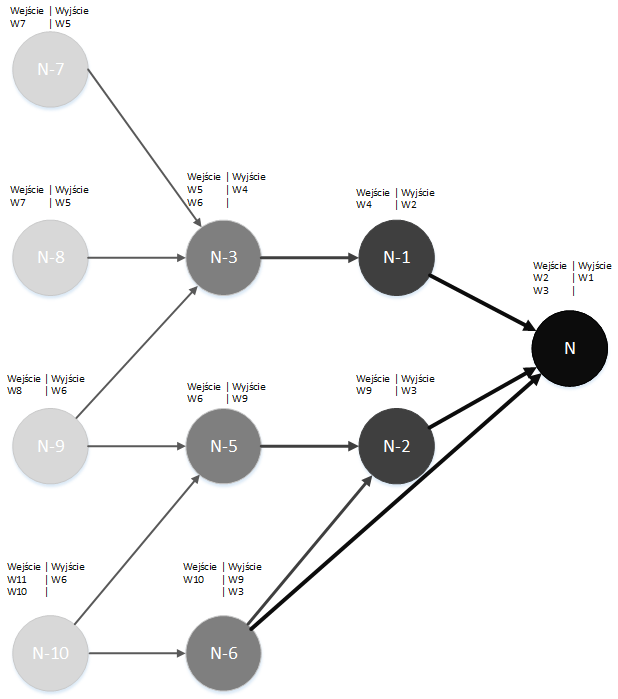
\includegraphics[height=\frameheight]{pictures/visio/siec.png}
 \end{figure}
\end{frame}

\begin{frame}
 \frametitle{Sposób budowy sieci}
 \framesubtitle{Praktyczny przykład}
  \begin{figure}
 		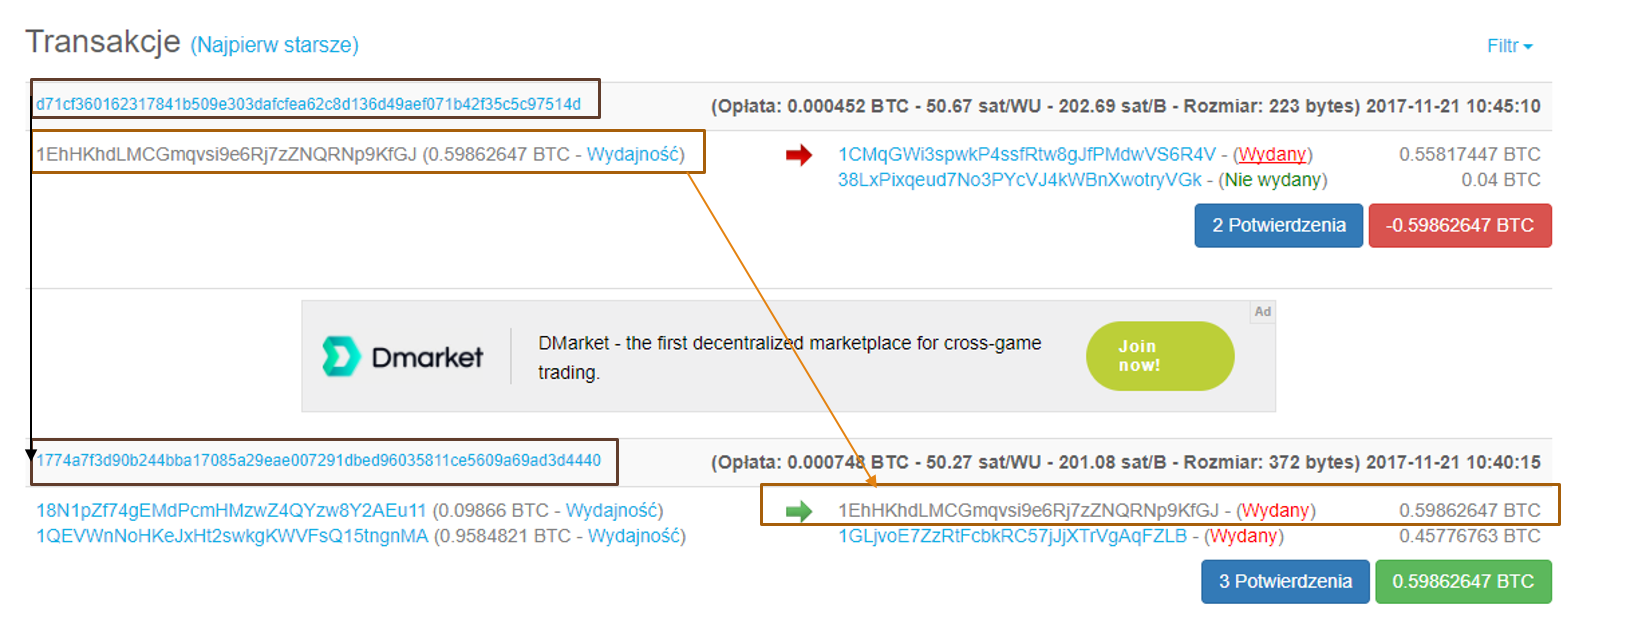
\includegraphics[width=1\linewidth]{pictures/transakcje.png}
	\end{figure}
\end{frame}

\begin{frame}
 \frametitle{Przykładowa sieć}
 \framesubtitle{}
  \begin{figure}
	\centering
 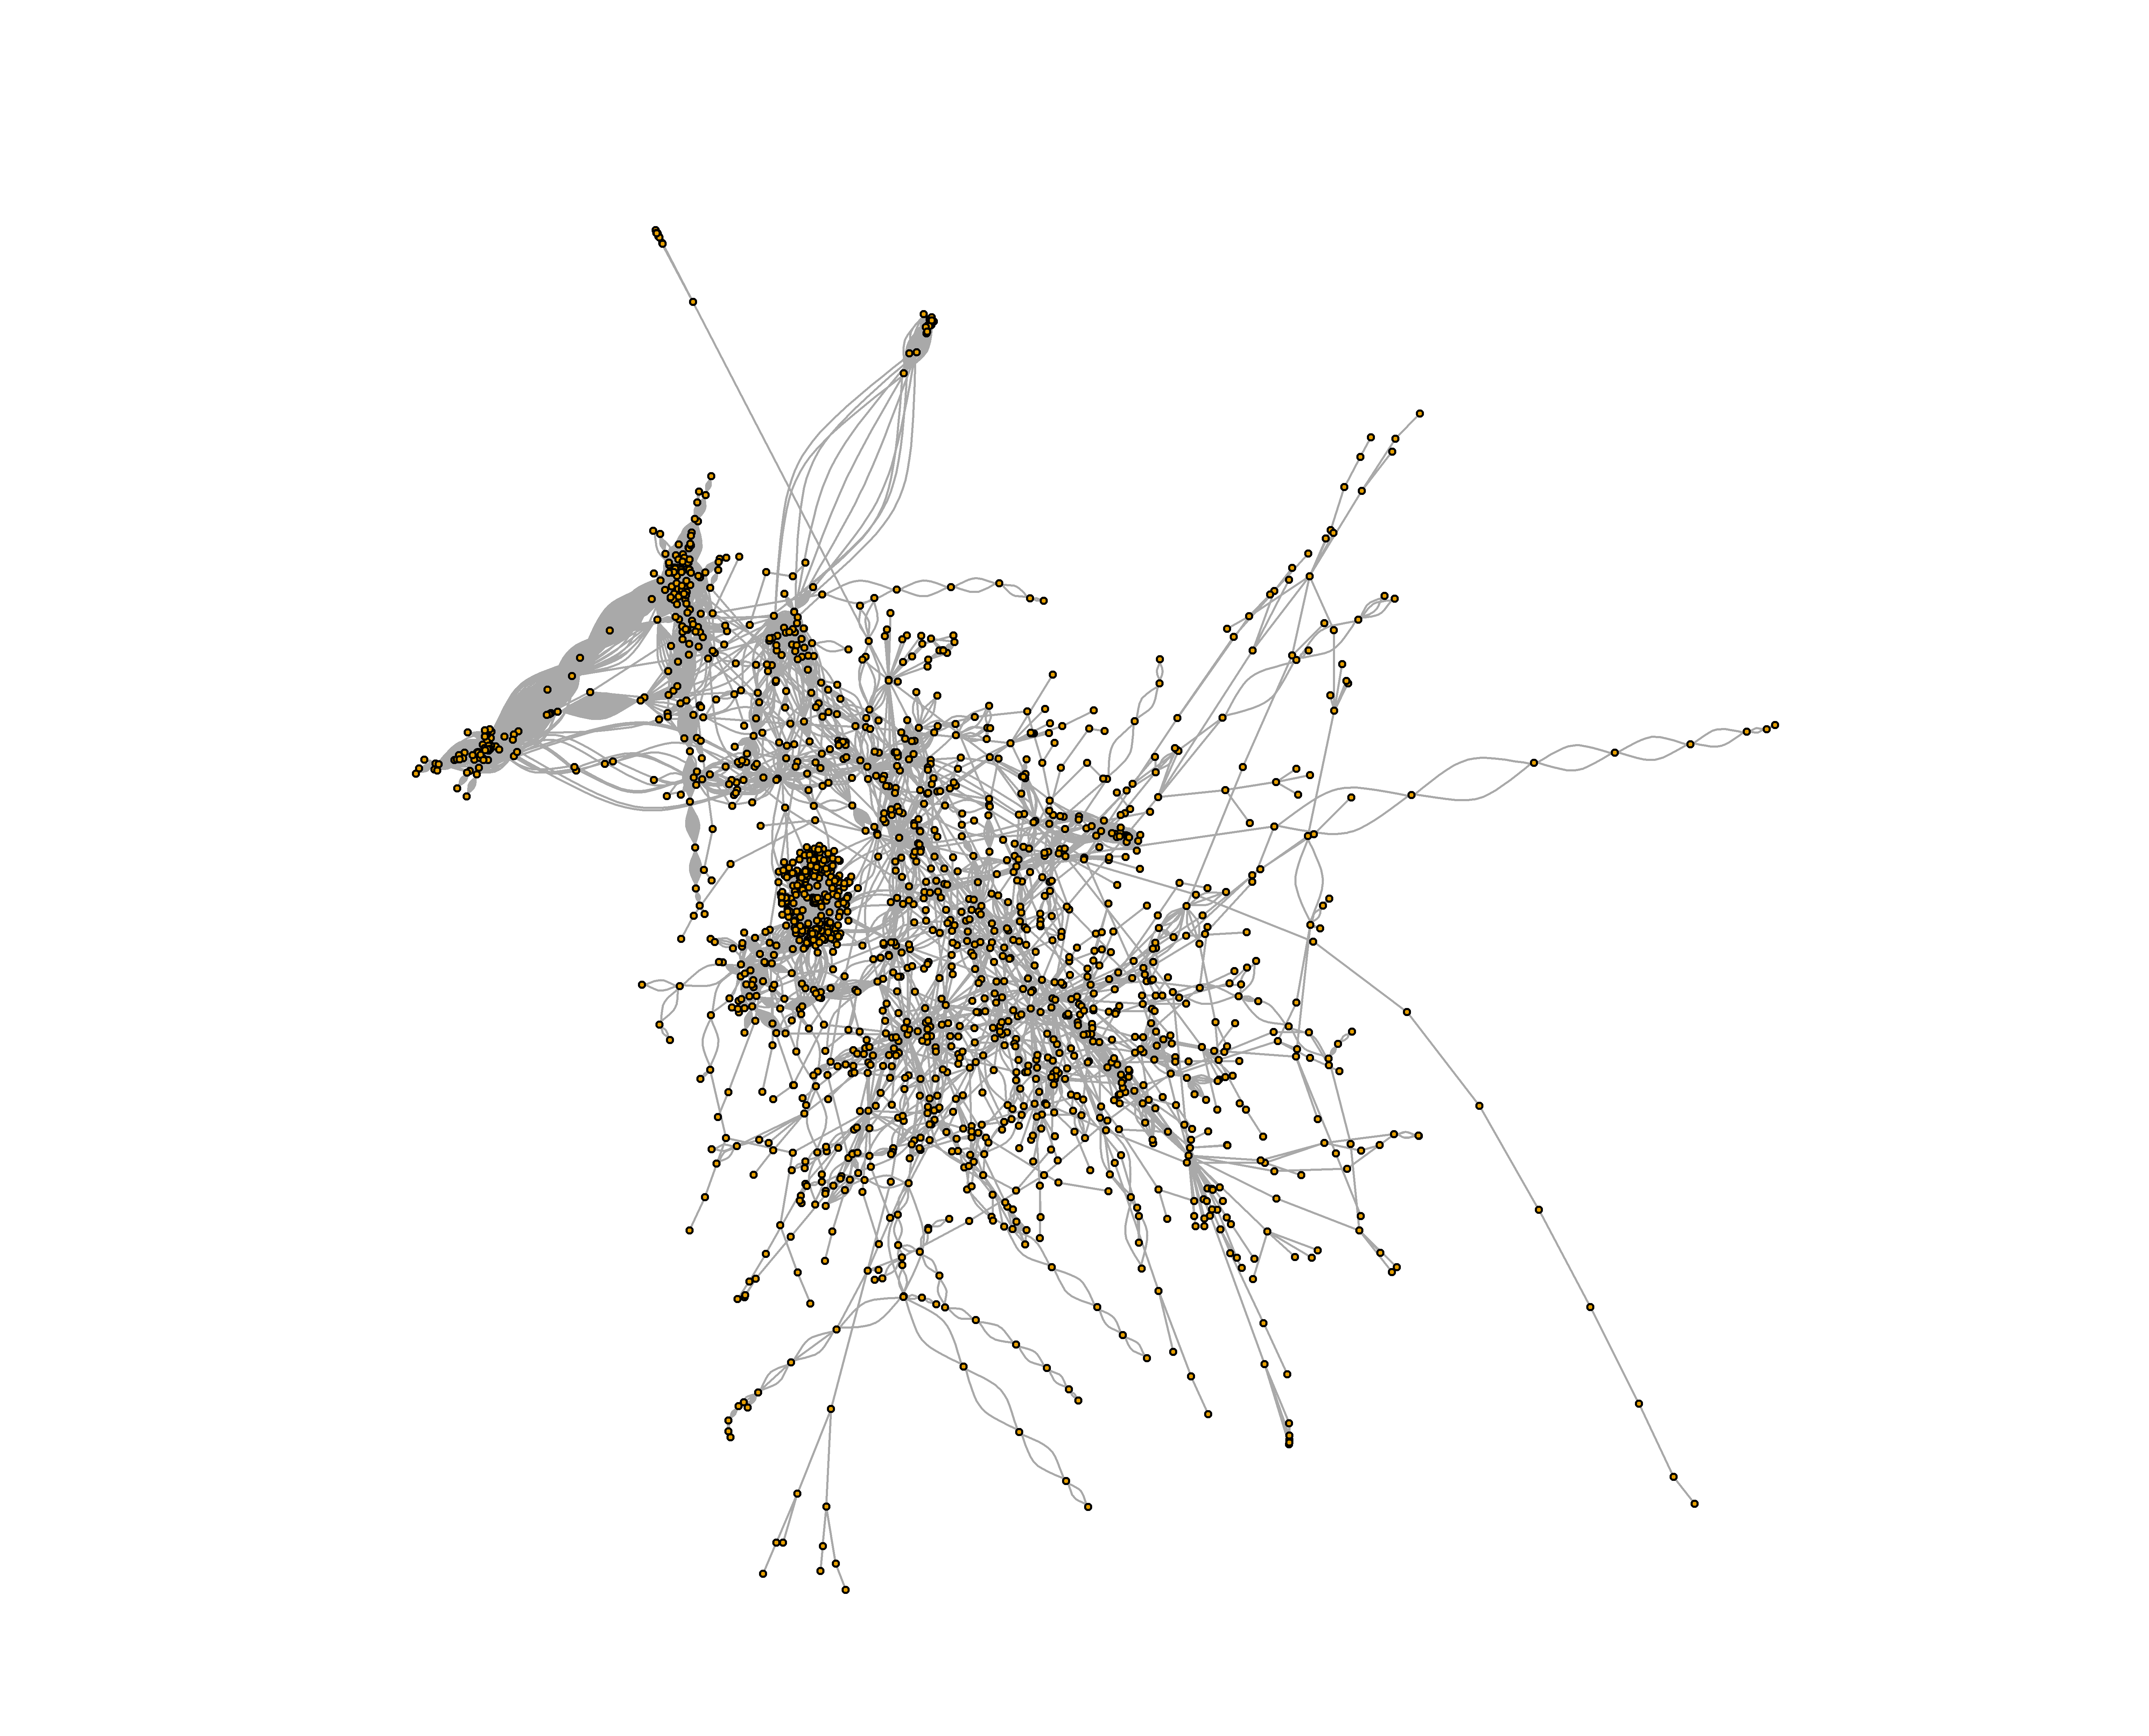
\includegraphics[height=\frameheight]{pictures/graph/graph.png}
  \end{figure}
\end{frame}


\begin{frame}
 \frametitle{Przeprowadzone badania}
 \framesubtitle{}
 \justify
Przeprowadzono badania podstawowych właściwości sieci:
\begin{itemize}
\item[--] średnicy,
\item[--] średniej długości ścieżek,
\item[--] średniego stopienia węzłów,
\item[--] średniej centralności węzłów,
\end{itemize}
oraz badania wynikające z jej specyfiki:
\begin{itemize}
\item[--] średnia wartość transakcji,
\item[--] liczba bloków potrzebnych do stworzenia próby,
\item[--] średnia różnica czasów kolejnych transakcji,
\item[--] różnica czasu granicznych transakcji.
\end{itemize}
\end{frame}

\begin{frame}
 \frametitle{Wyniki}
 \framesubtitle{Generyczne właściwości sieci}
  \begin{minipage}{\textwidth}
     \centering
 			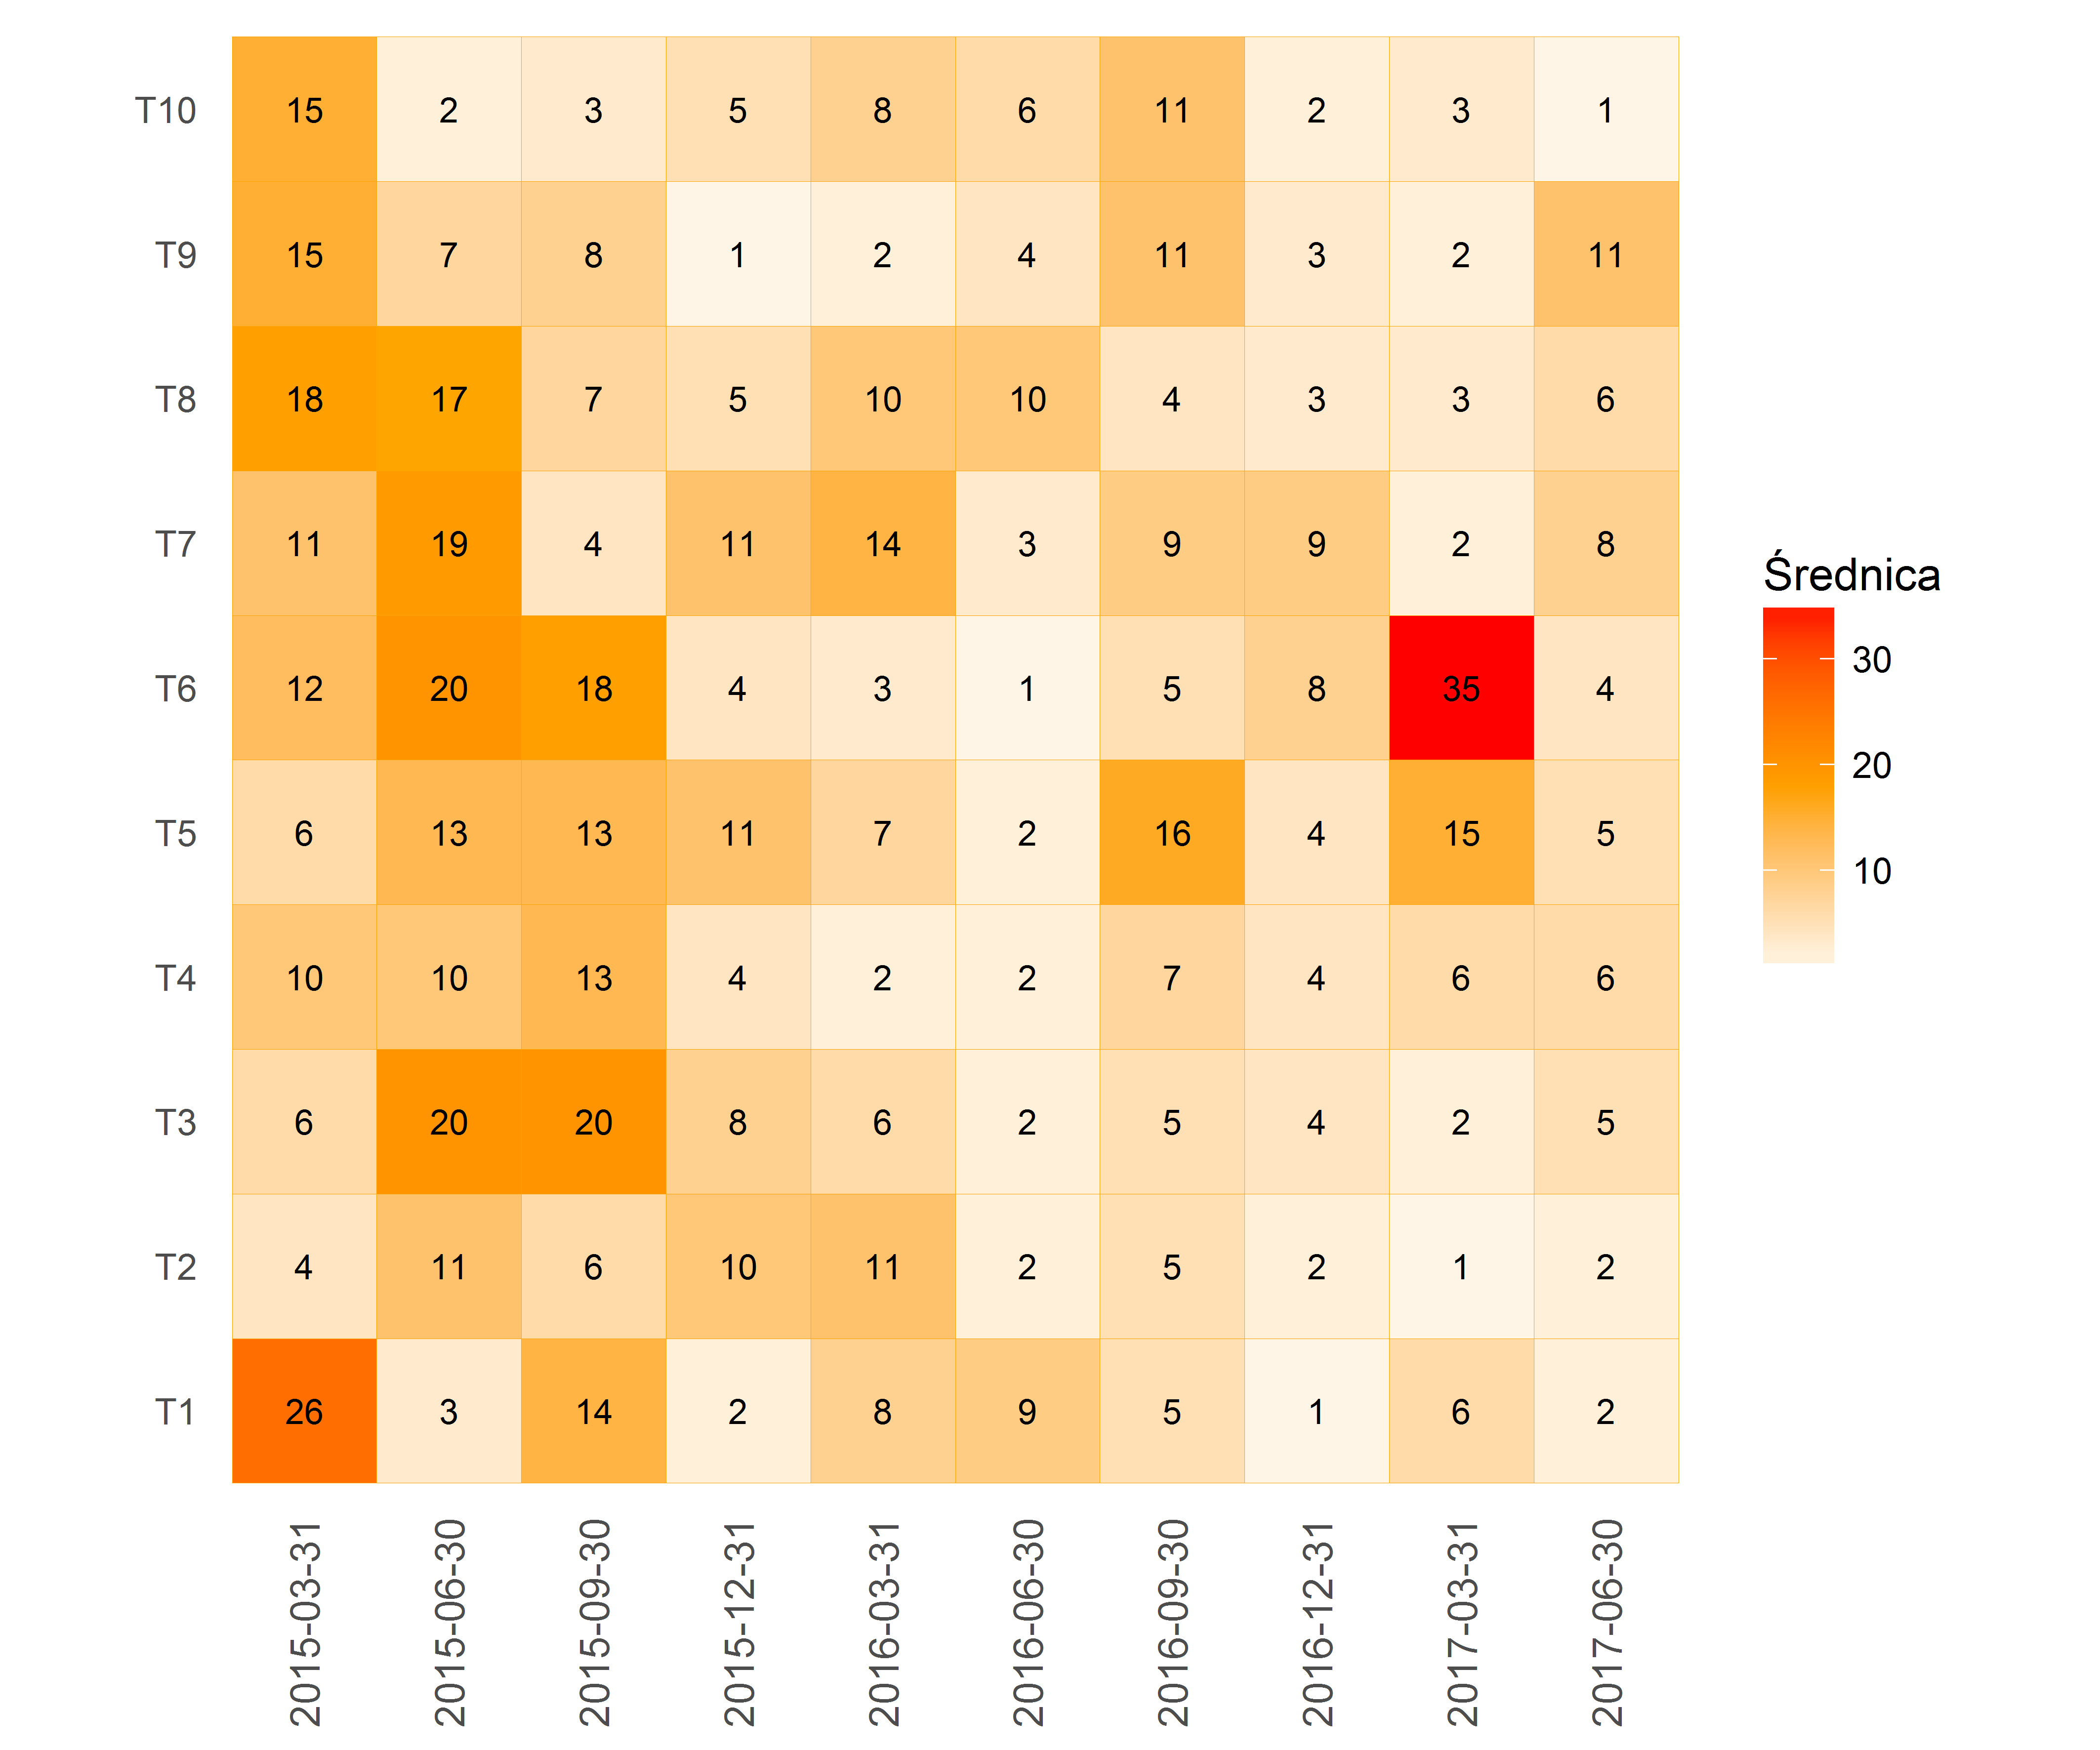
\includegraphics[width=\sizequad\textwidth]{pictures/srednica/srednica_hm.png}\quad  
            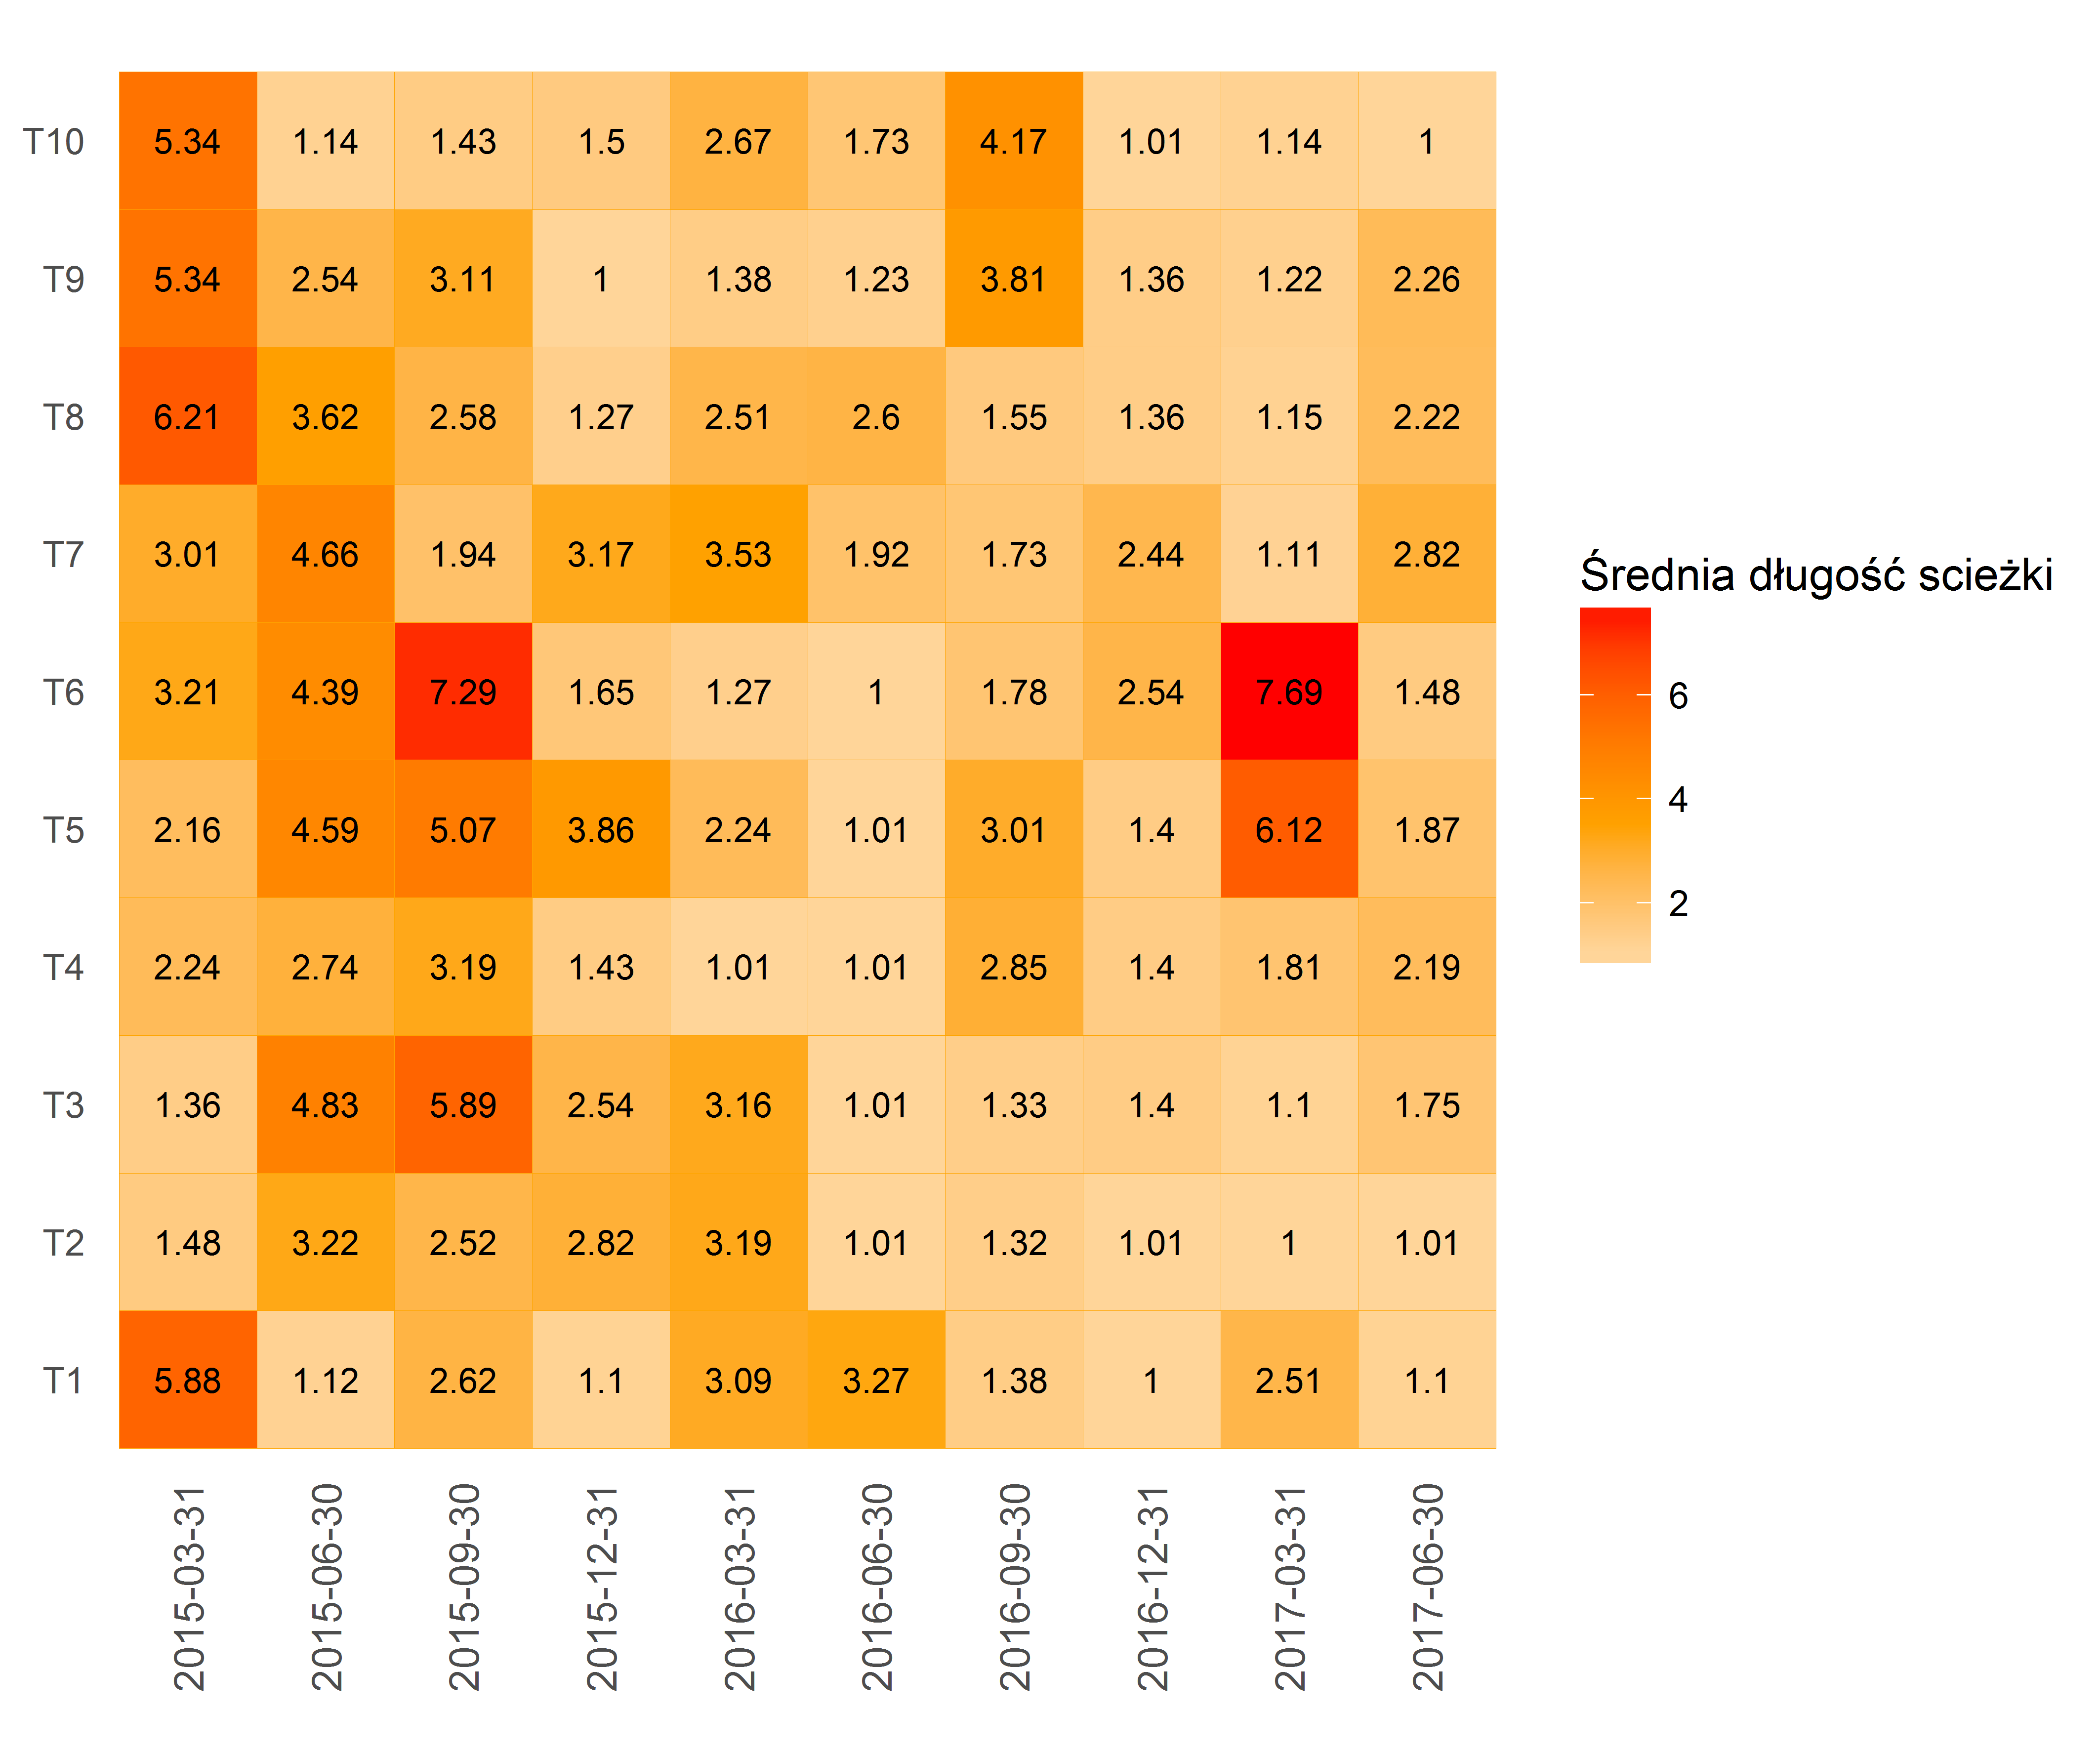
\includegraphics[width=\sizequad\textwidth]{pictures/srednia_dlugosc_sciezki/srednia_dlugosc_sciezki_hm.png}  \\
            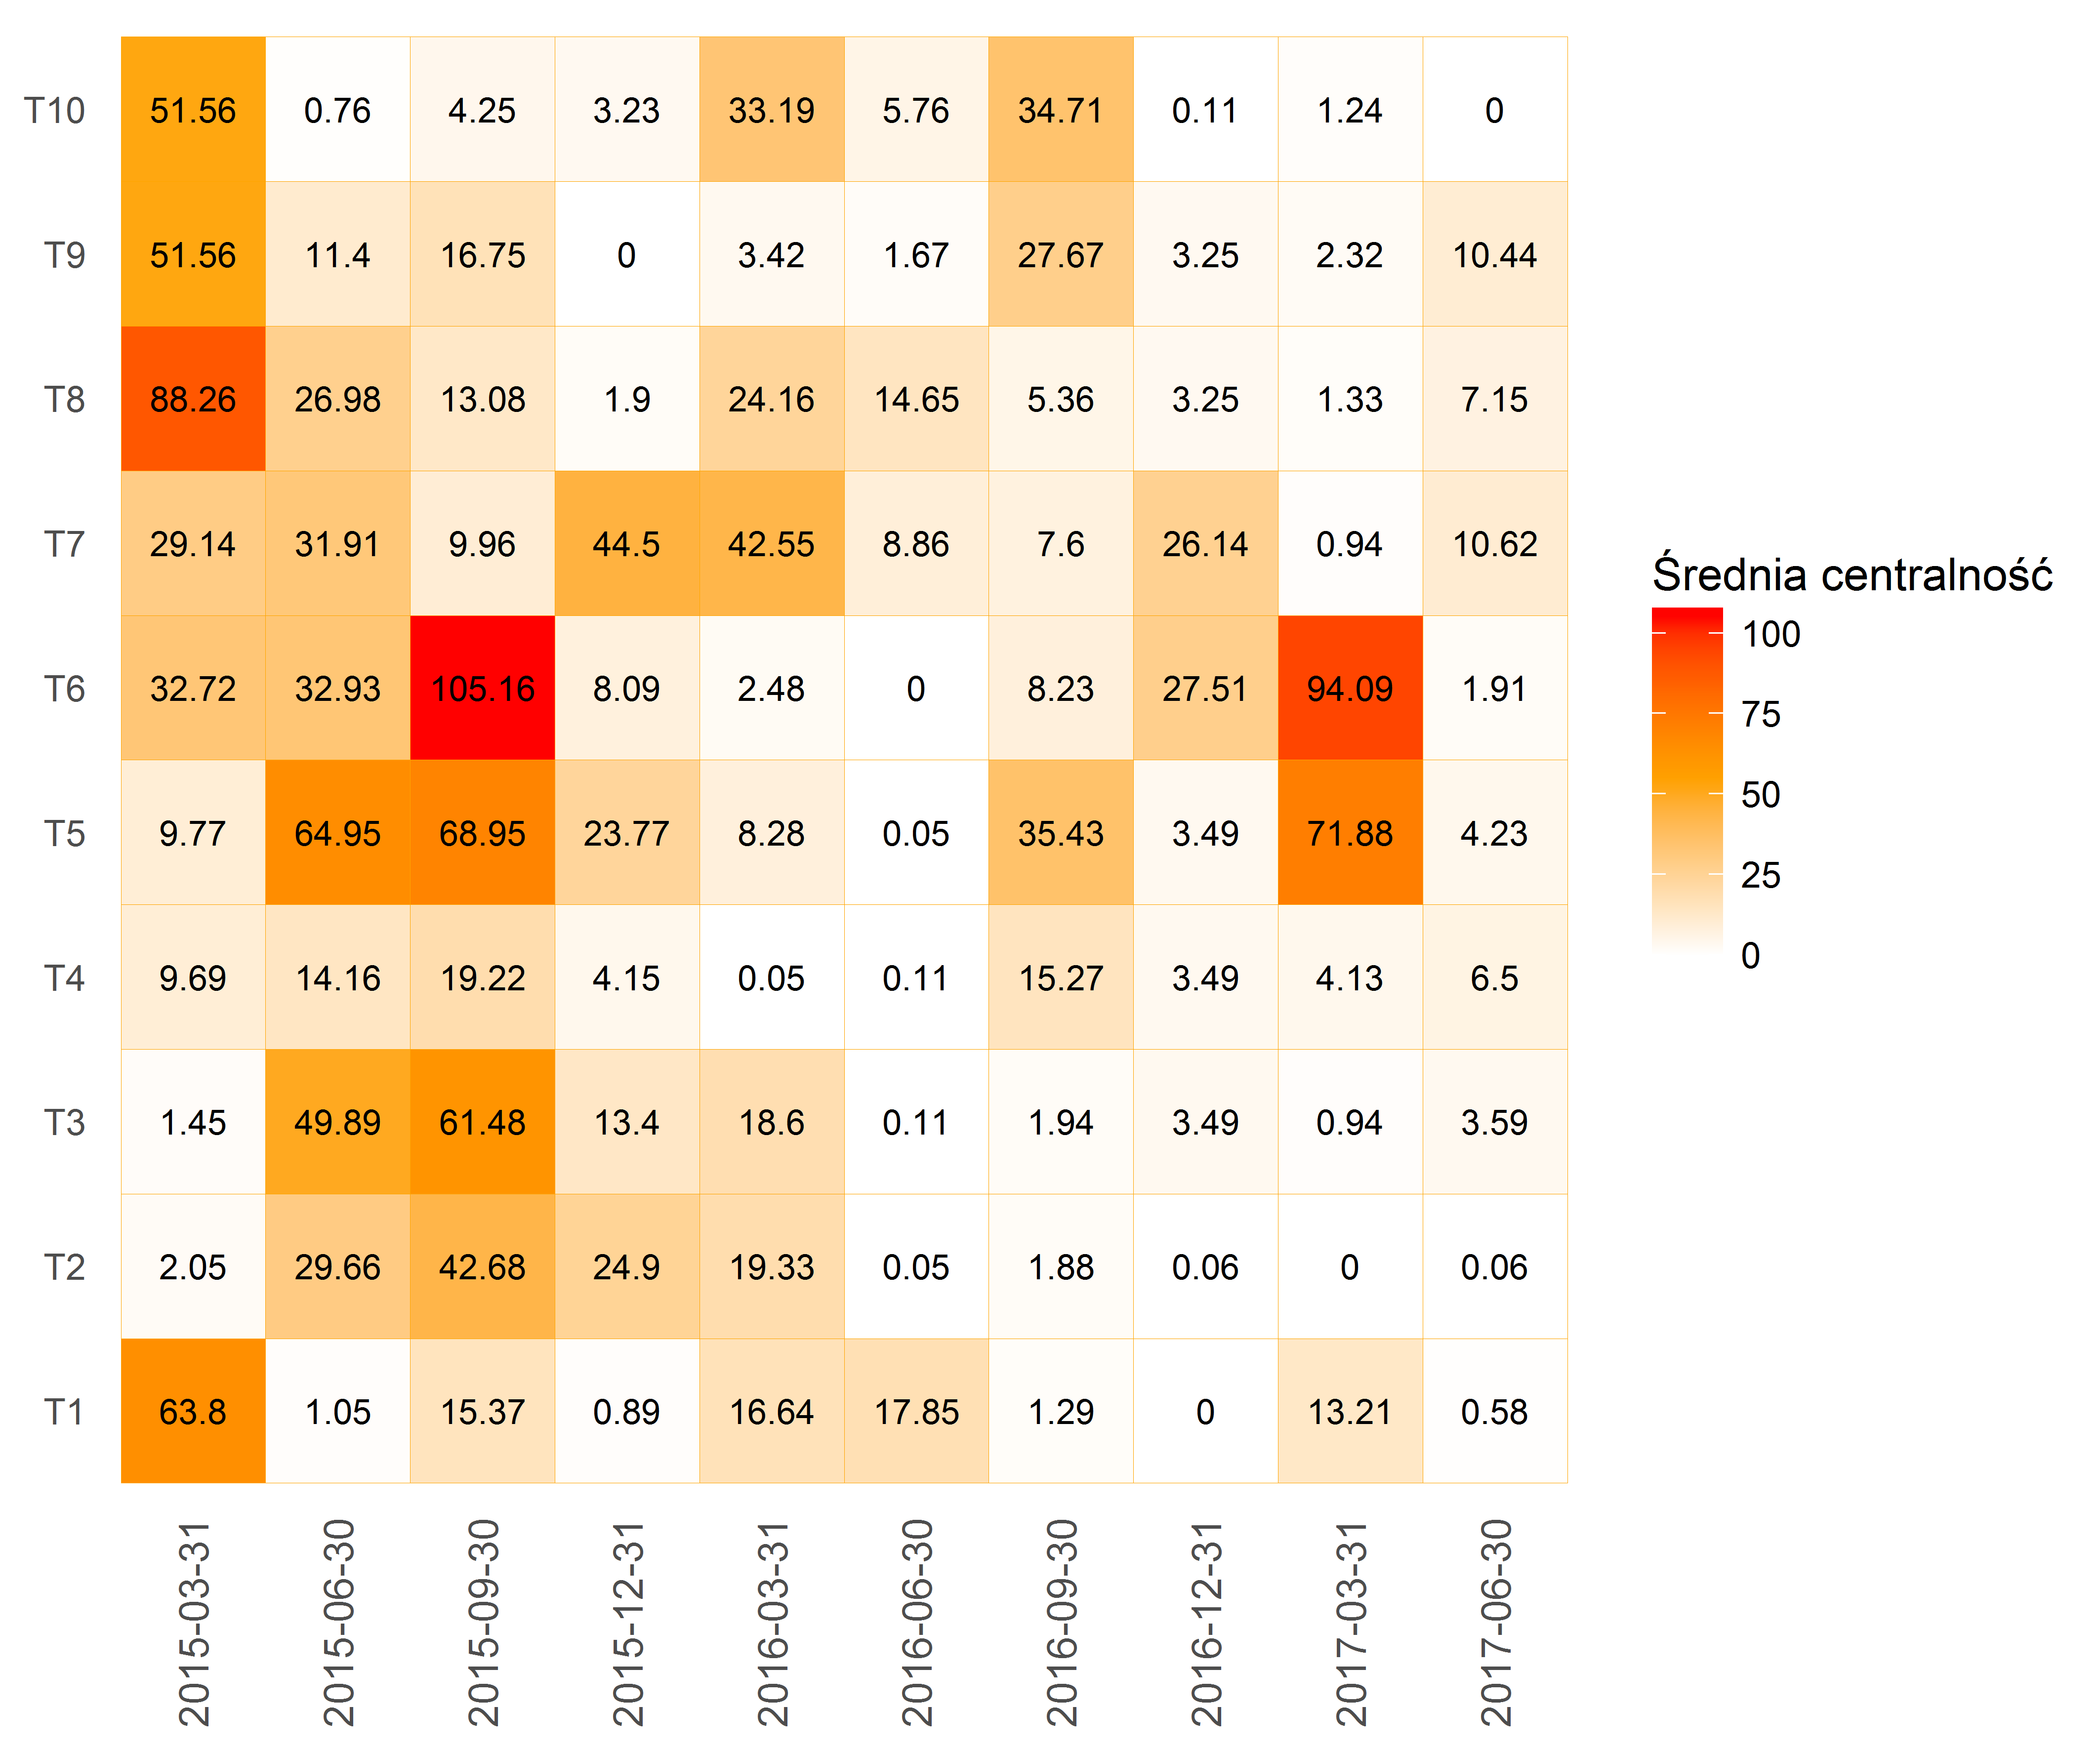
\includegraphics[width=\sizequad\textwidth]{pictures/srednia_centralnosc/srednia_centralnosc_hm.png}\quad
			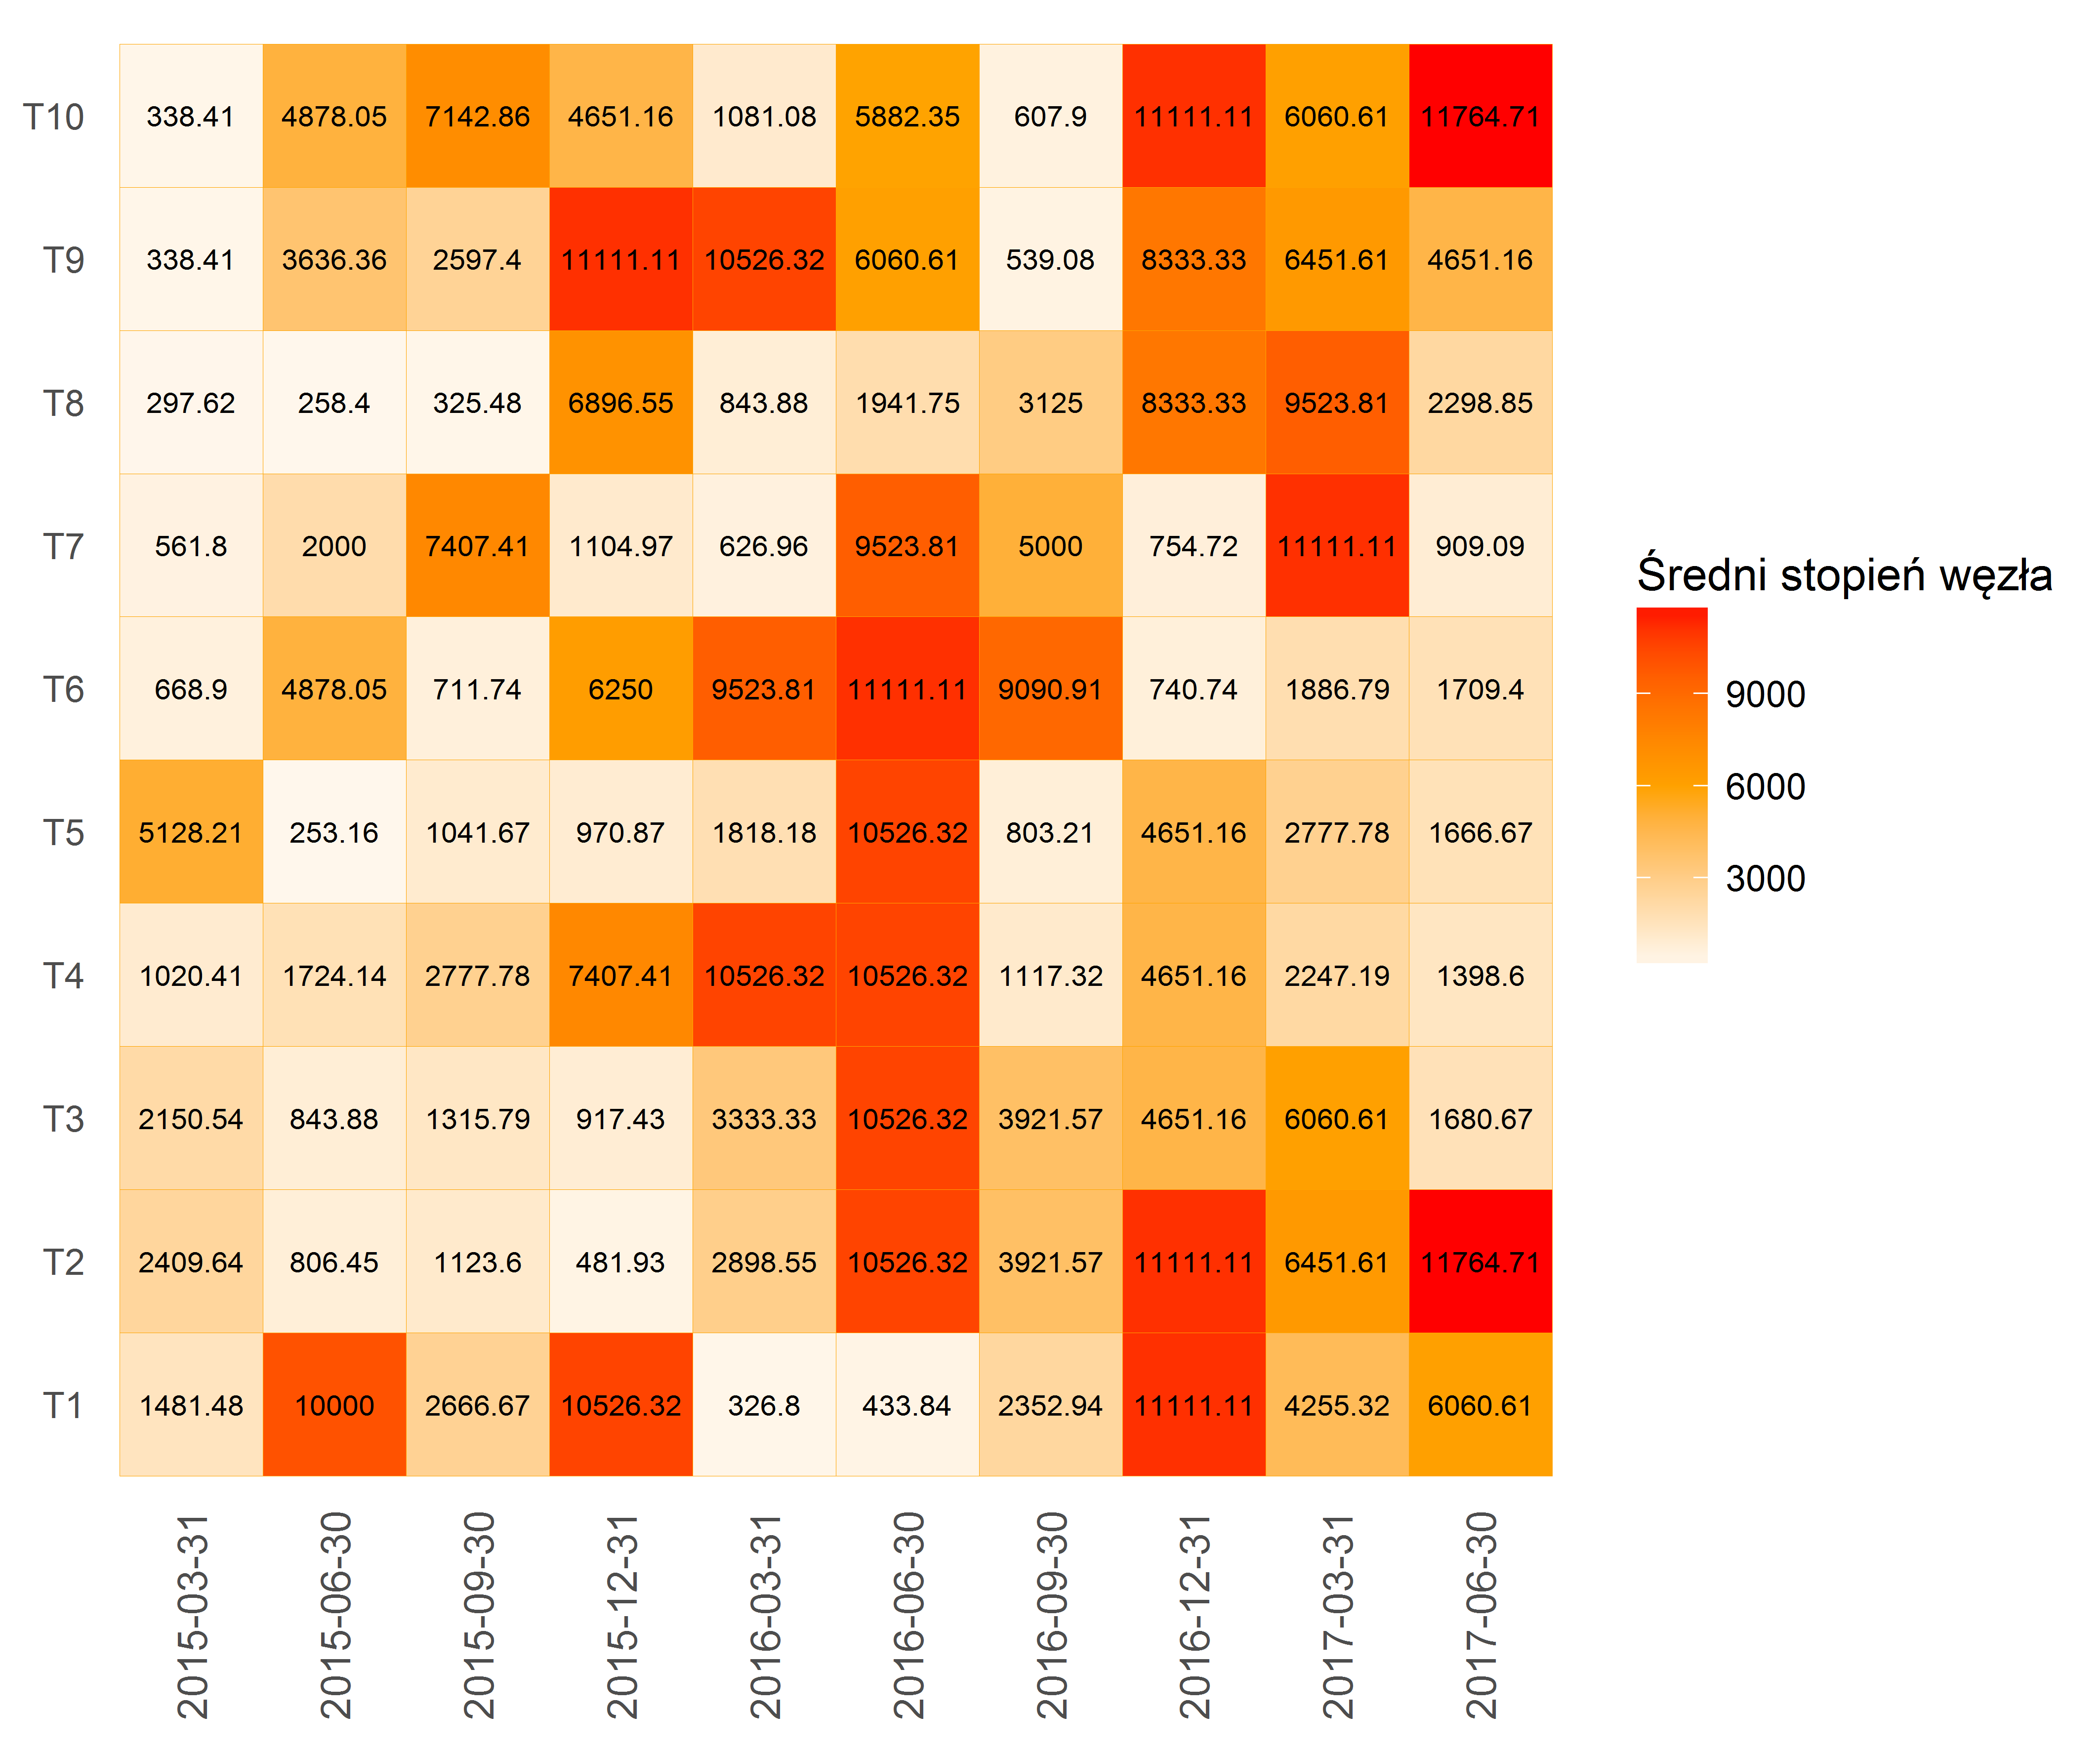
\includegraphics[width=\sizequad\textwidth]{pictures/sredni_stopien_wezla/sredni_stopien_wezla_hm.png}
 \end{minipage} 
 
\end{frame}

\begin{frame}
 \frametitle{Trend}
 \framesubtitle{Generyczne właściwości sieci}
 
  \begin{minipage}{\textwidth}
     \centering
 			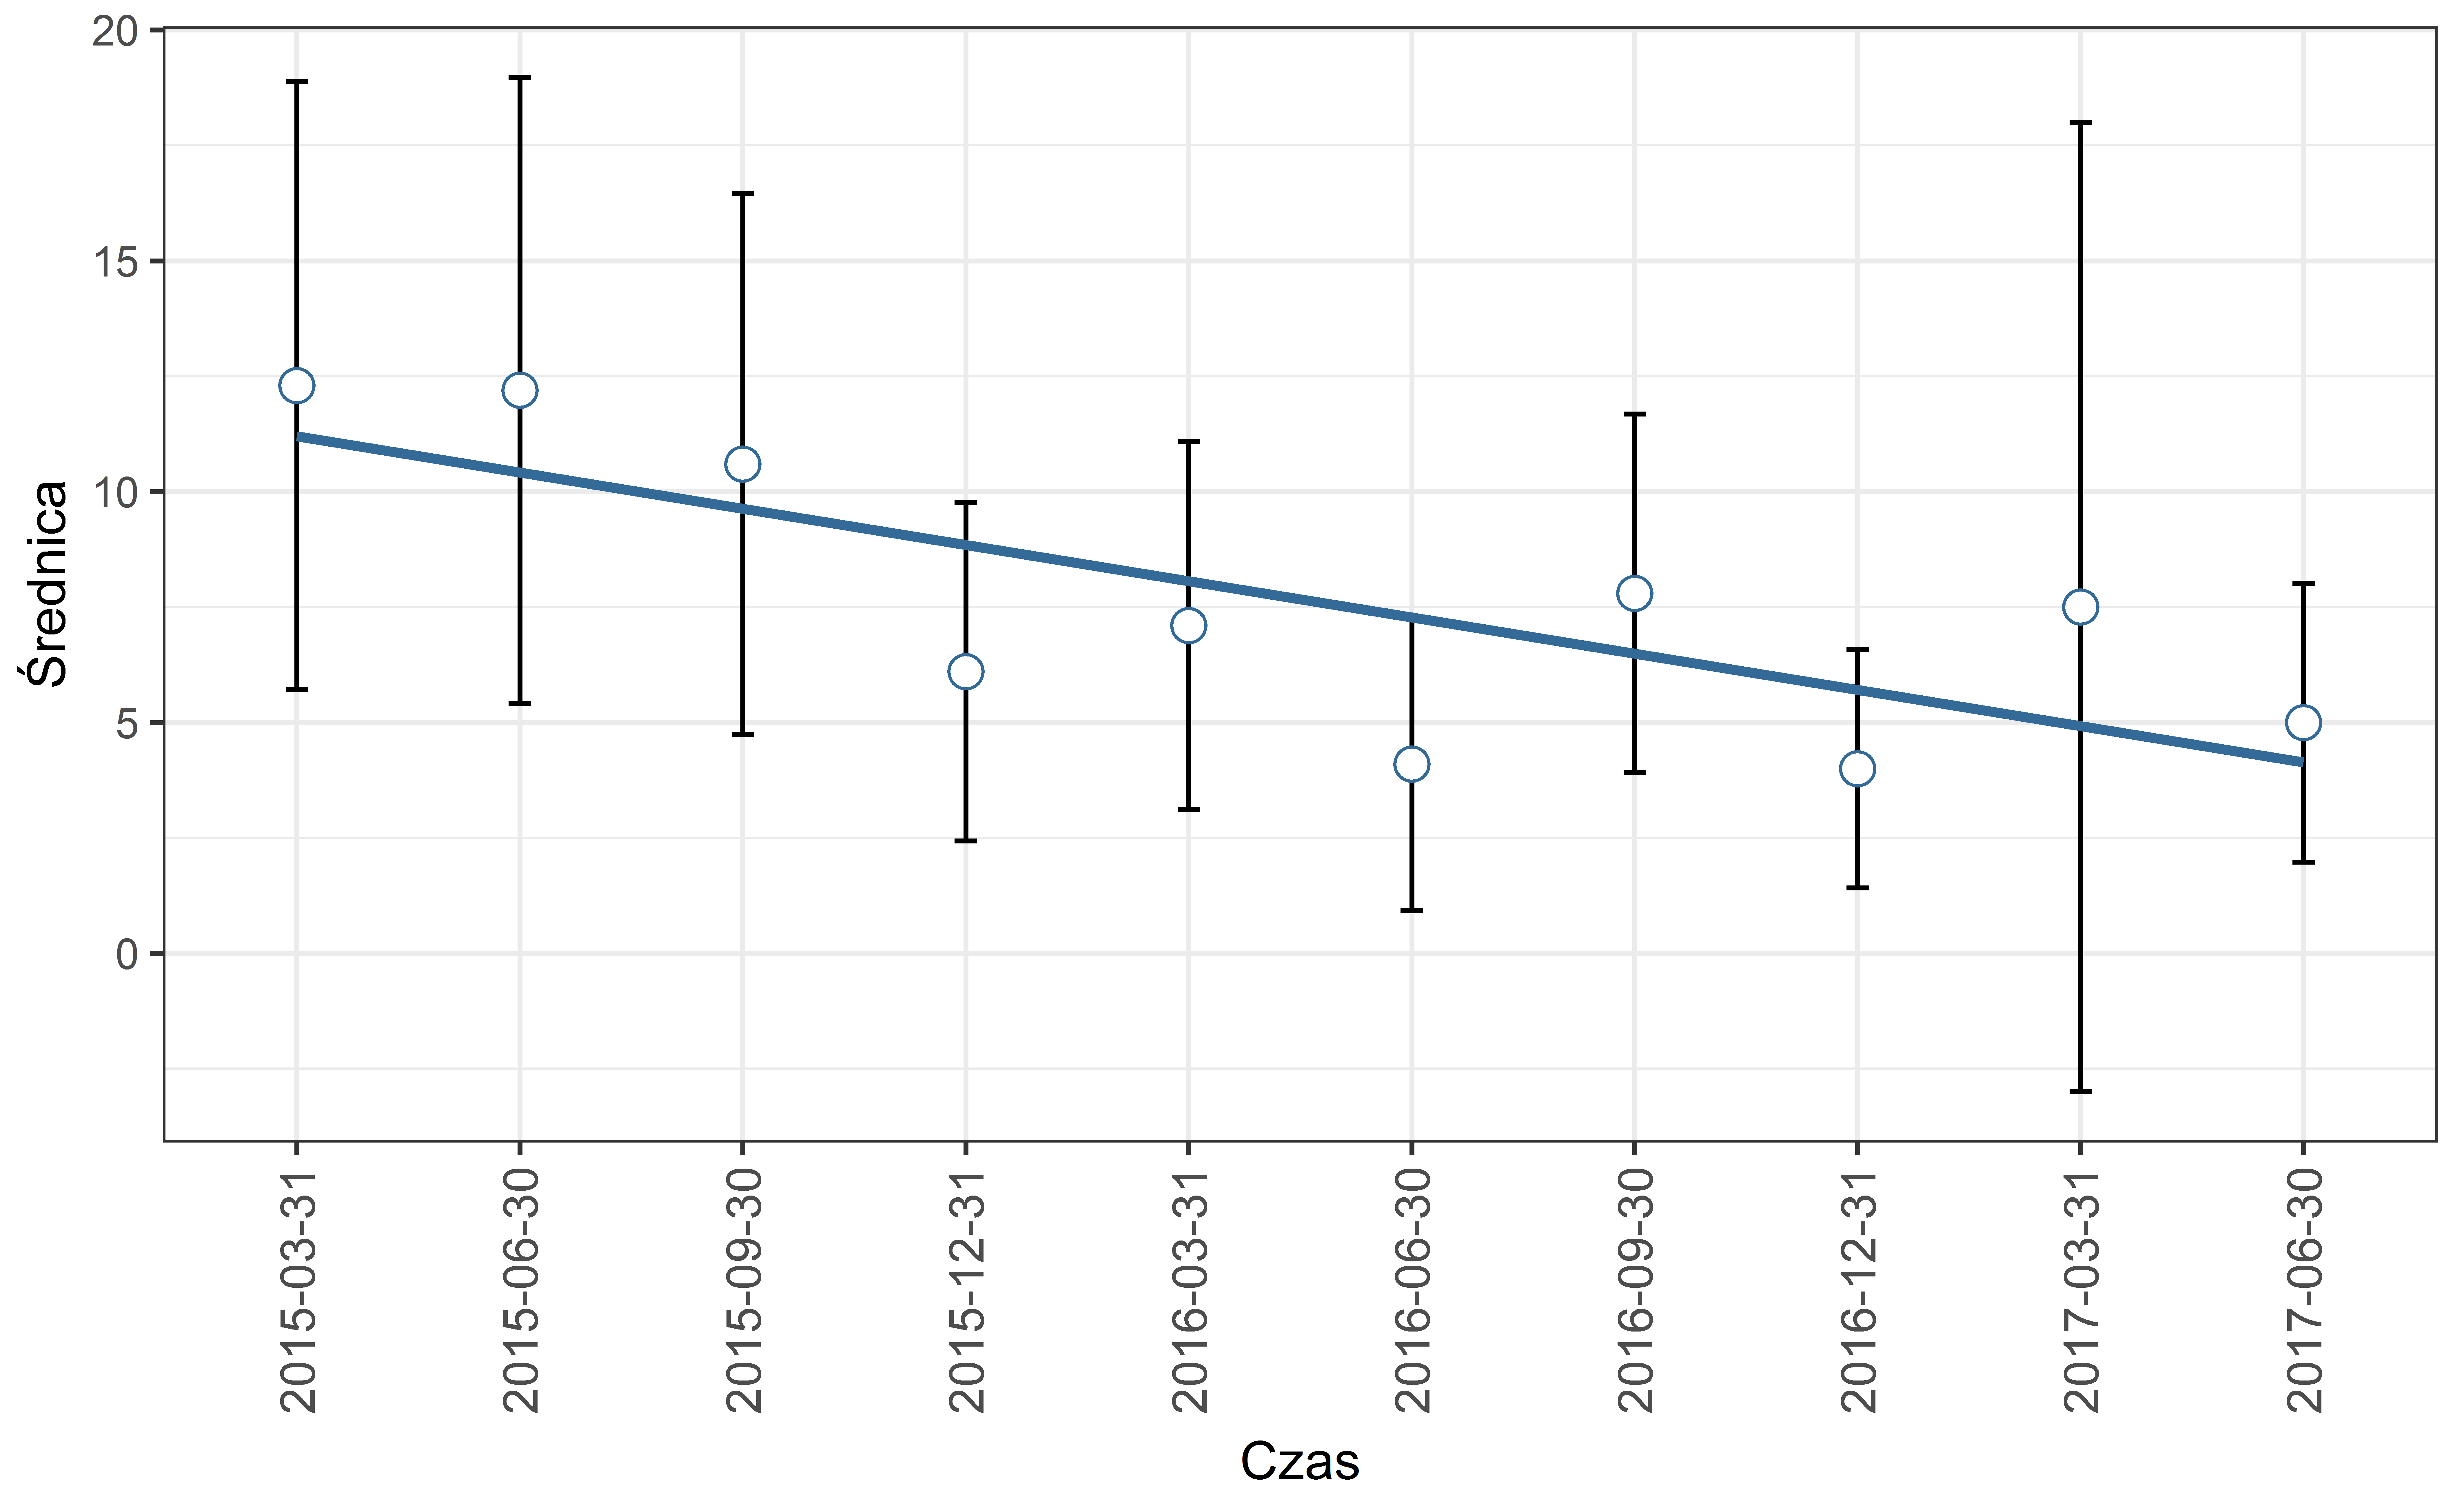
\includegraphics[width=\sizequadsda\textwidth]{pictures/srednica/srednica_sda.png}\quad  
            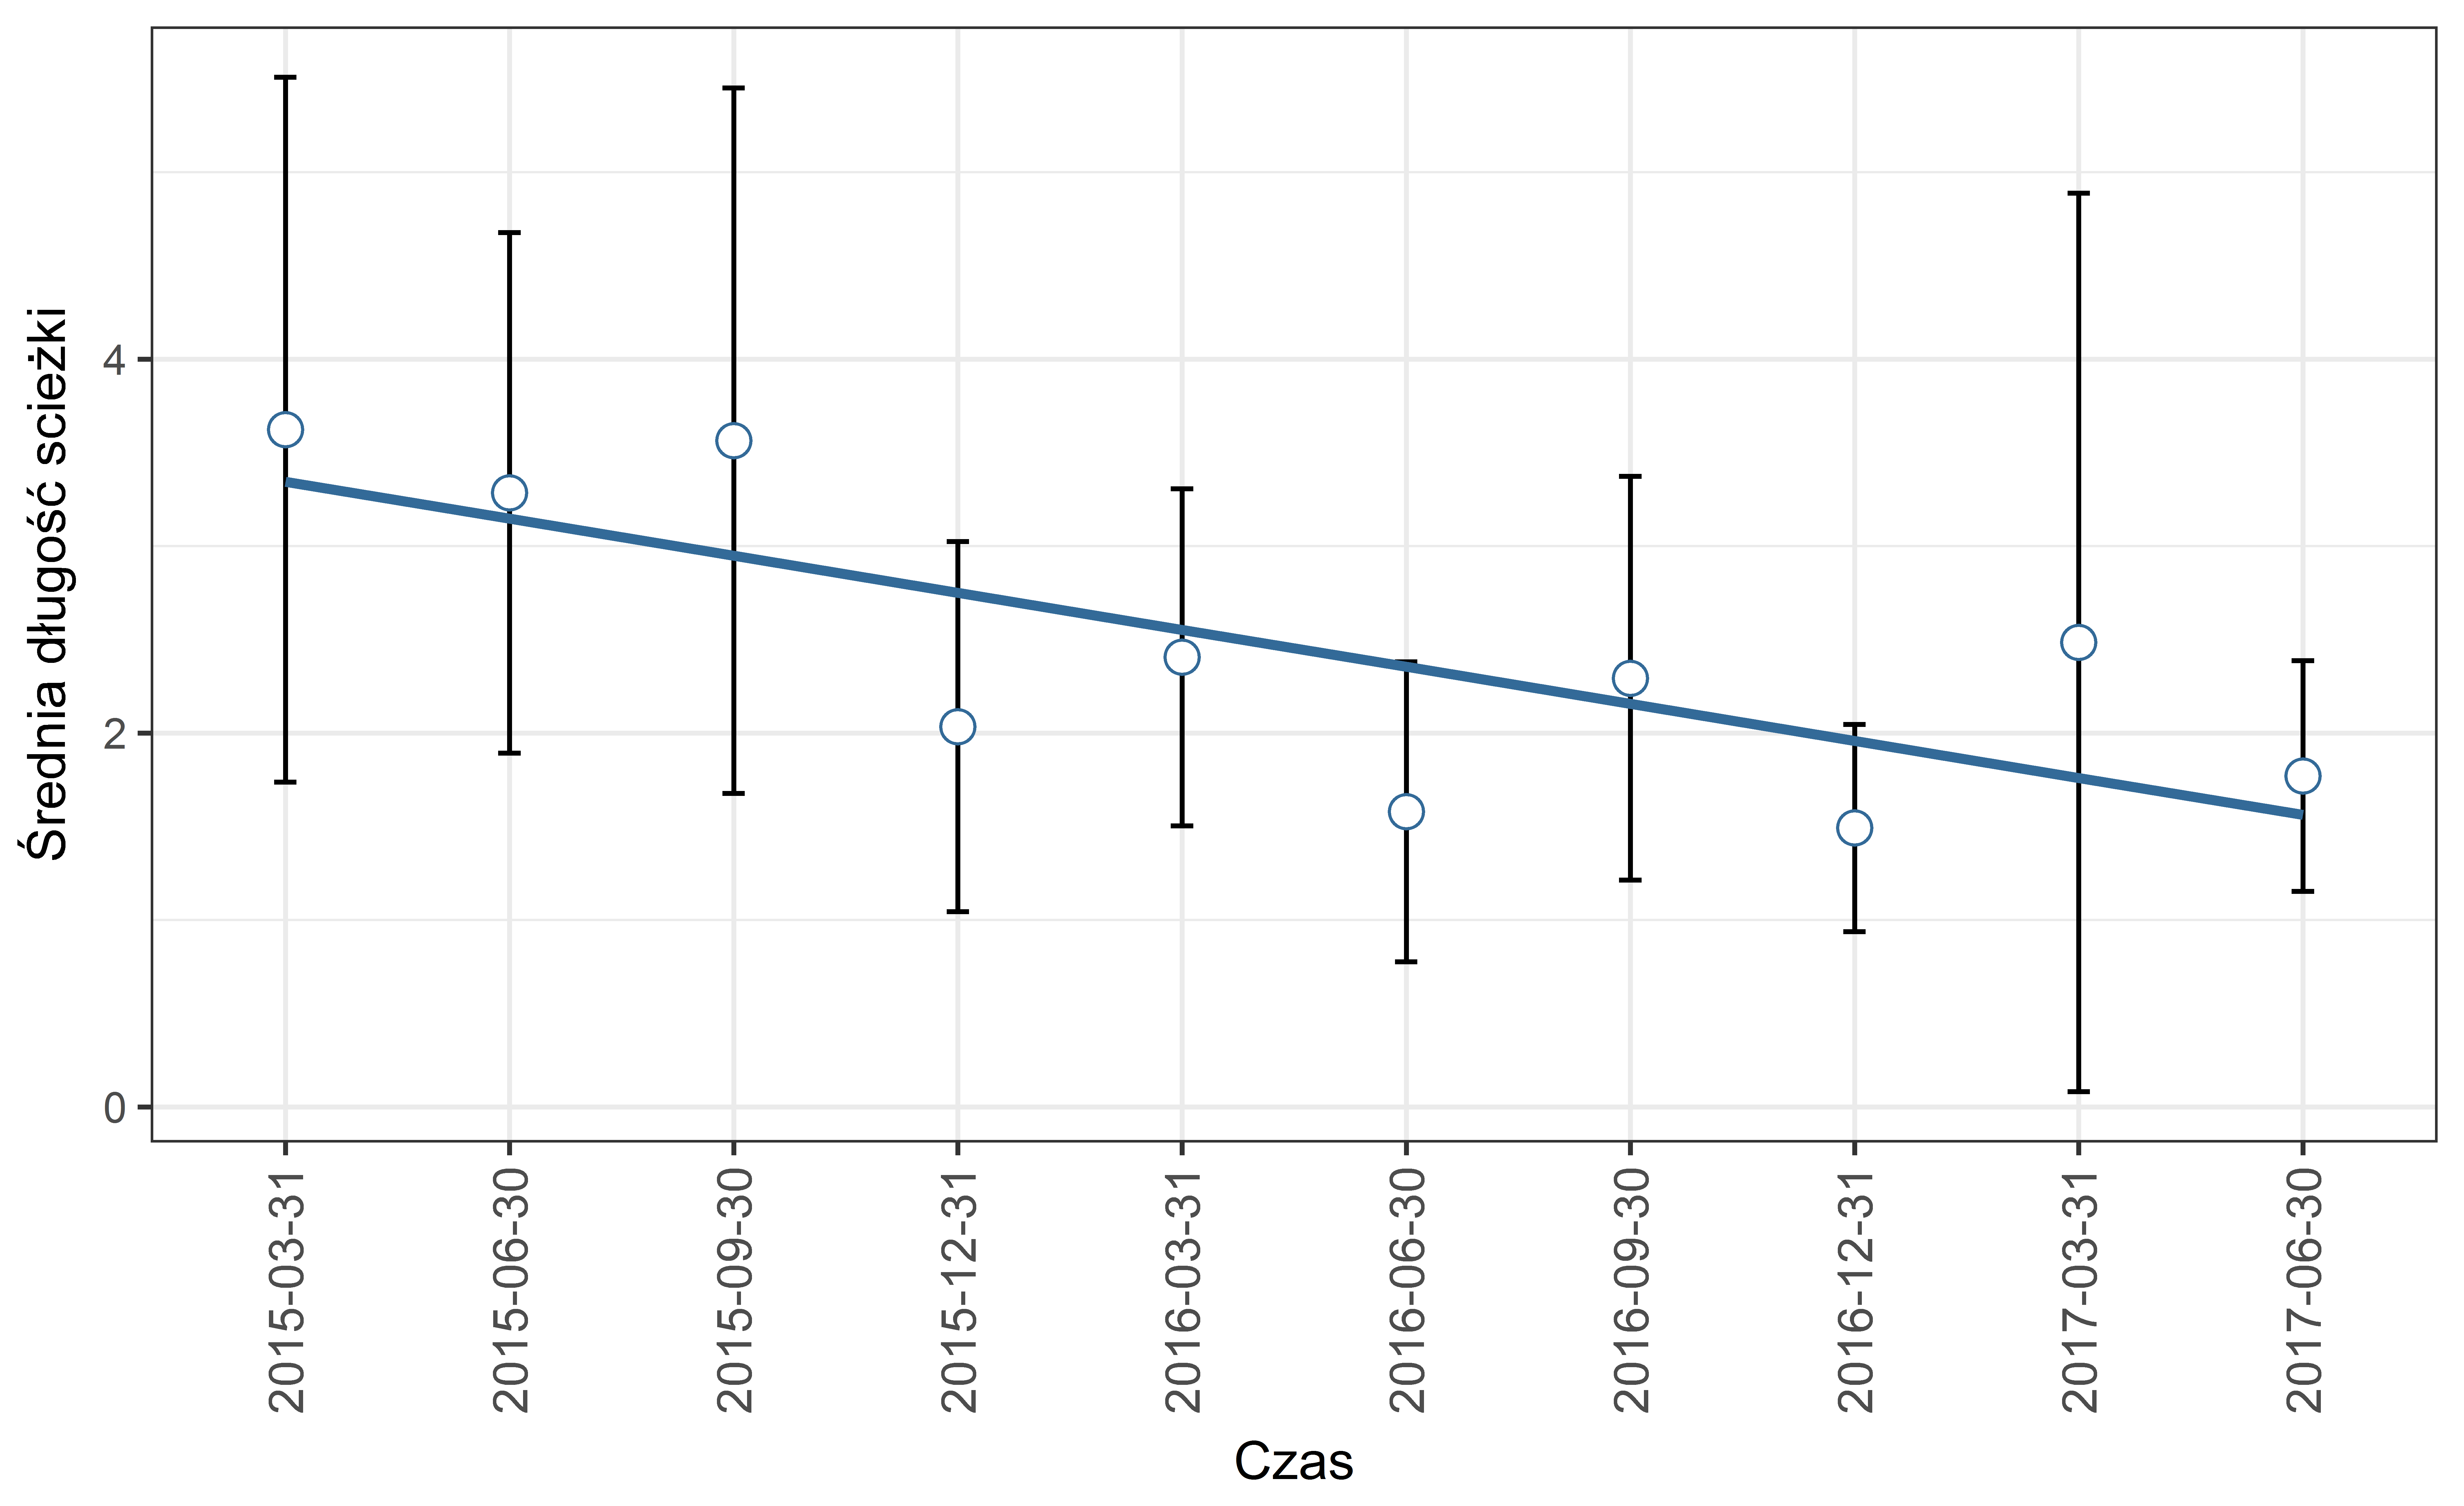
\includegraphics[width=\sizequadsda\textwidth]{pictures/srednia_dlugosc_sciezki/srednia_dlugosc_sciezki_sda.png}  \\
            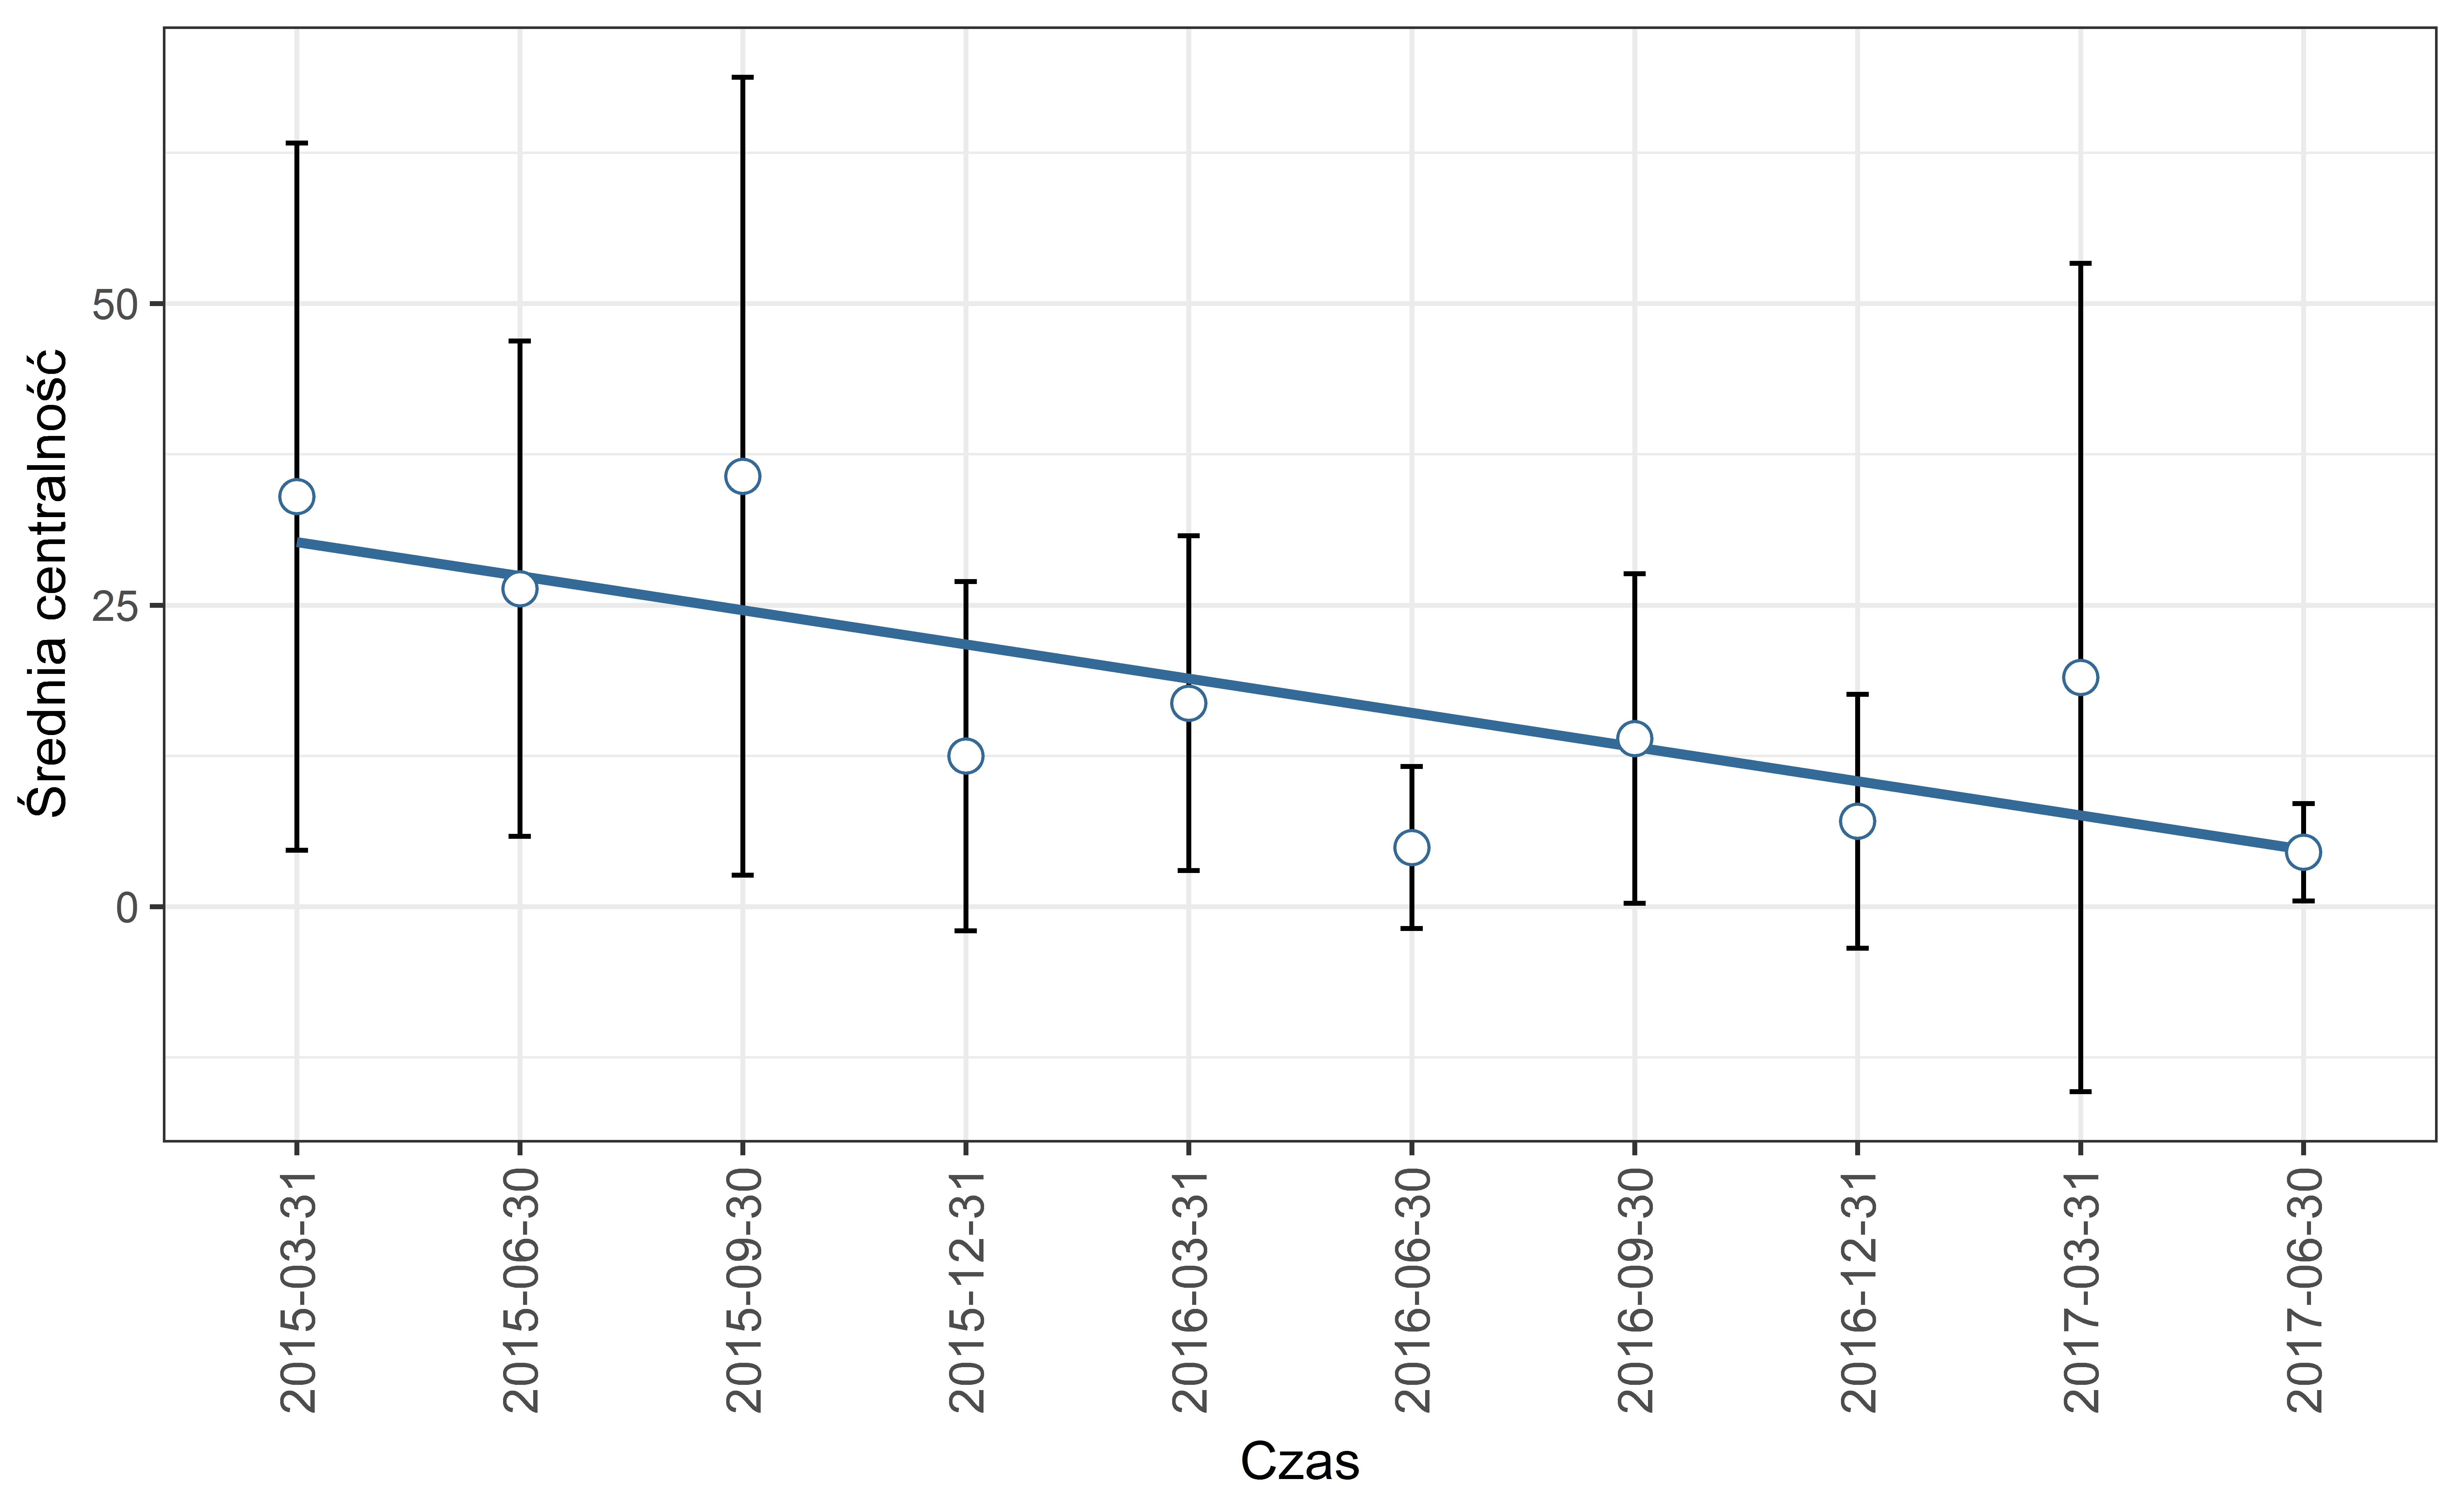
\includegraphics[width=\sizequadsda\textwidth]{pictures/srednia_centralnosc/srednia_centralnosc_sda.png}\quad
			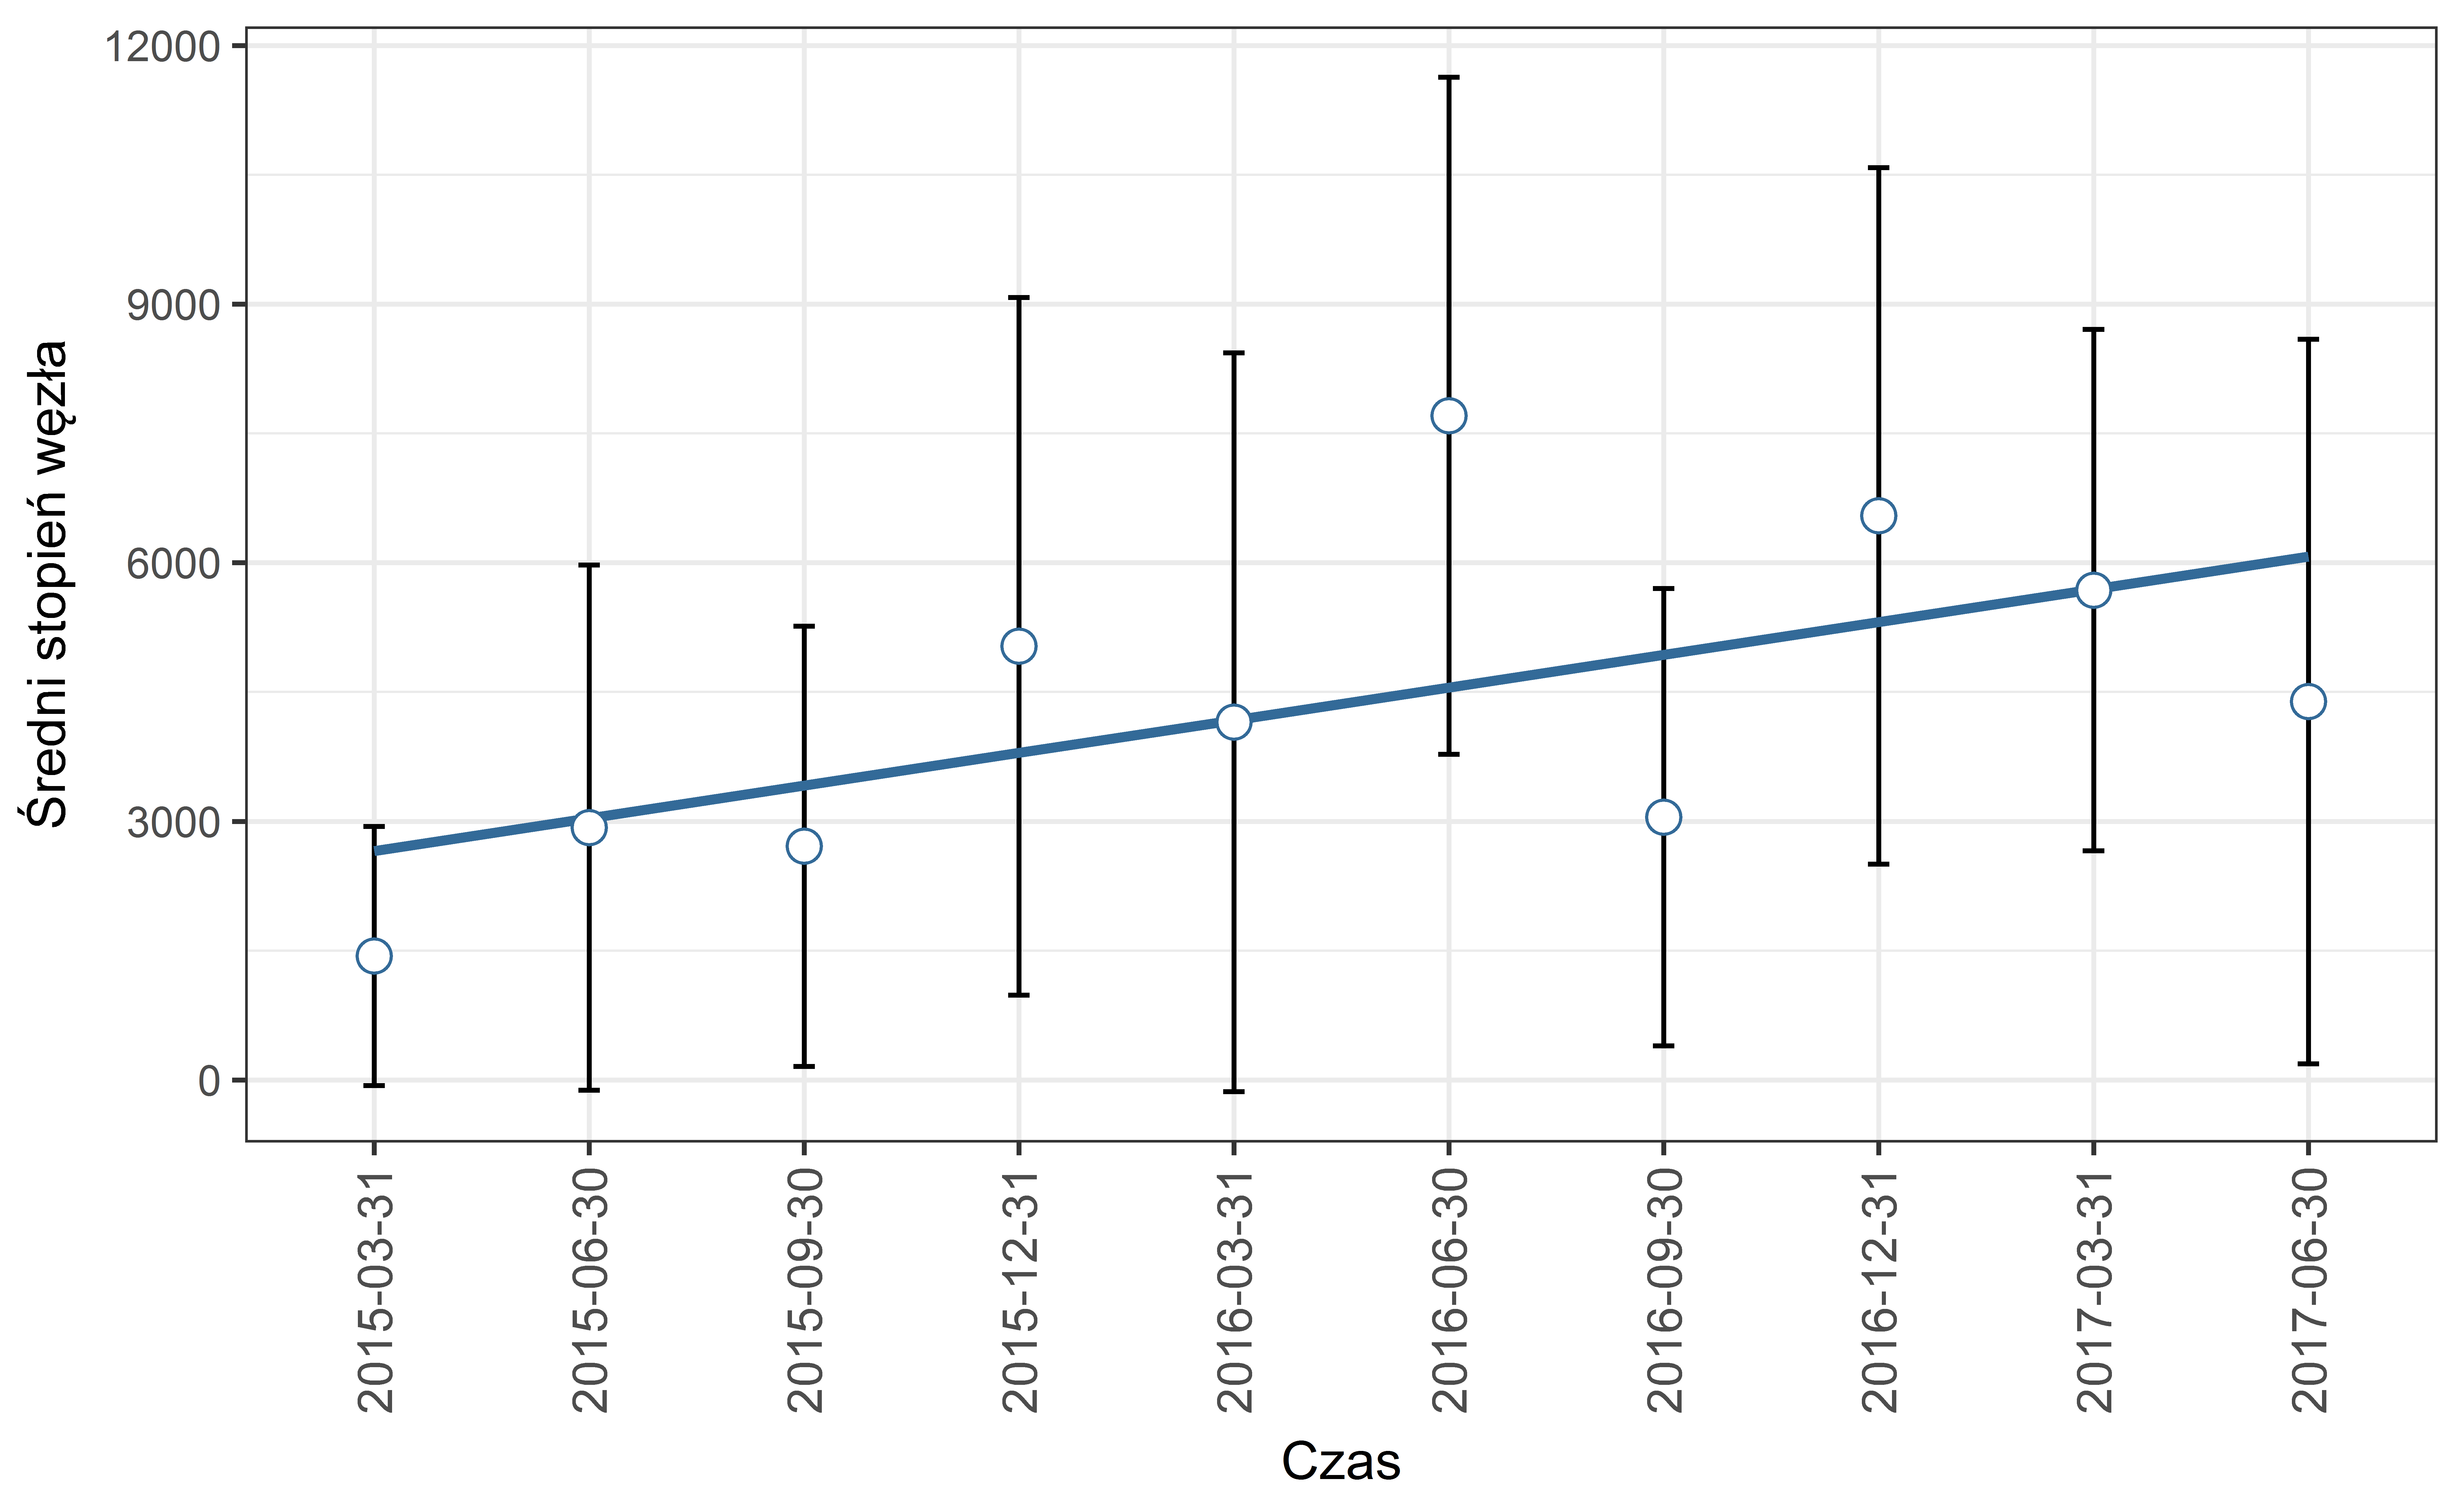
\includegraphics[width=\sizequadsda\textwidth]{pictures/sredni_stopien_wezla/sredni_stopien_wezla_sda.png}
 \end{minipage} 
\end{frame}

\begin{frame}
 \frametitle{Wyniki}
 \framesubtitle{Własności sieci wynikające z jej specyfiki}
   \begin{minipage}{\textwidth}
     \centering
 		  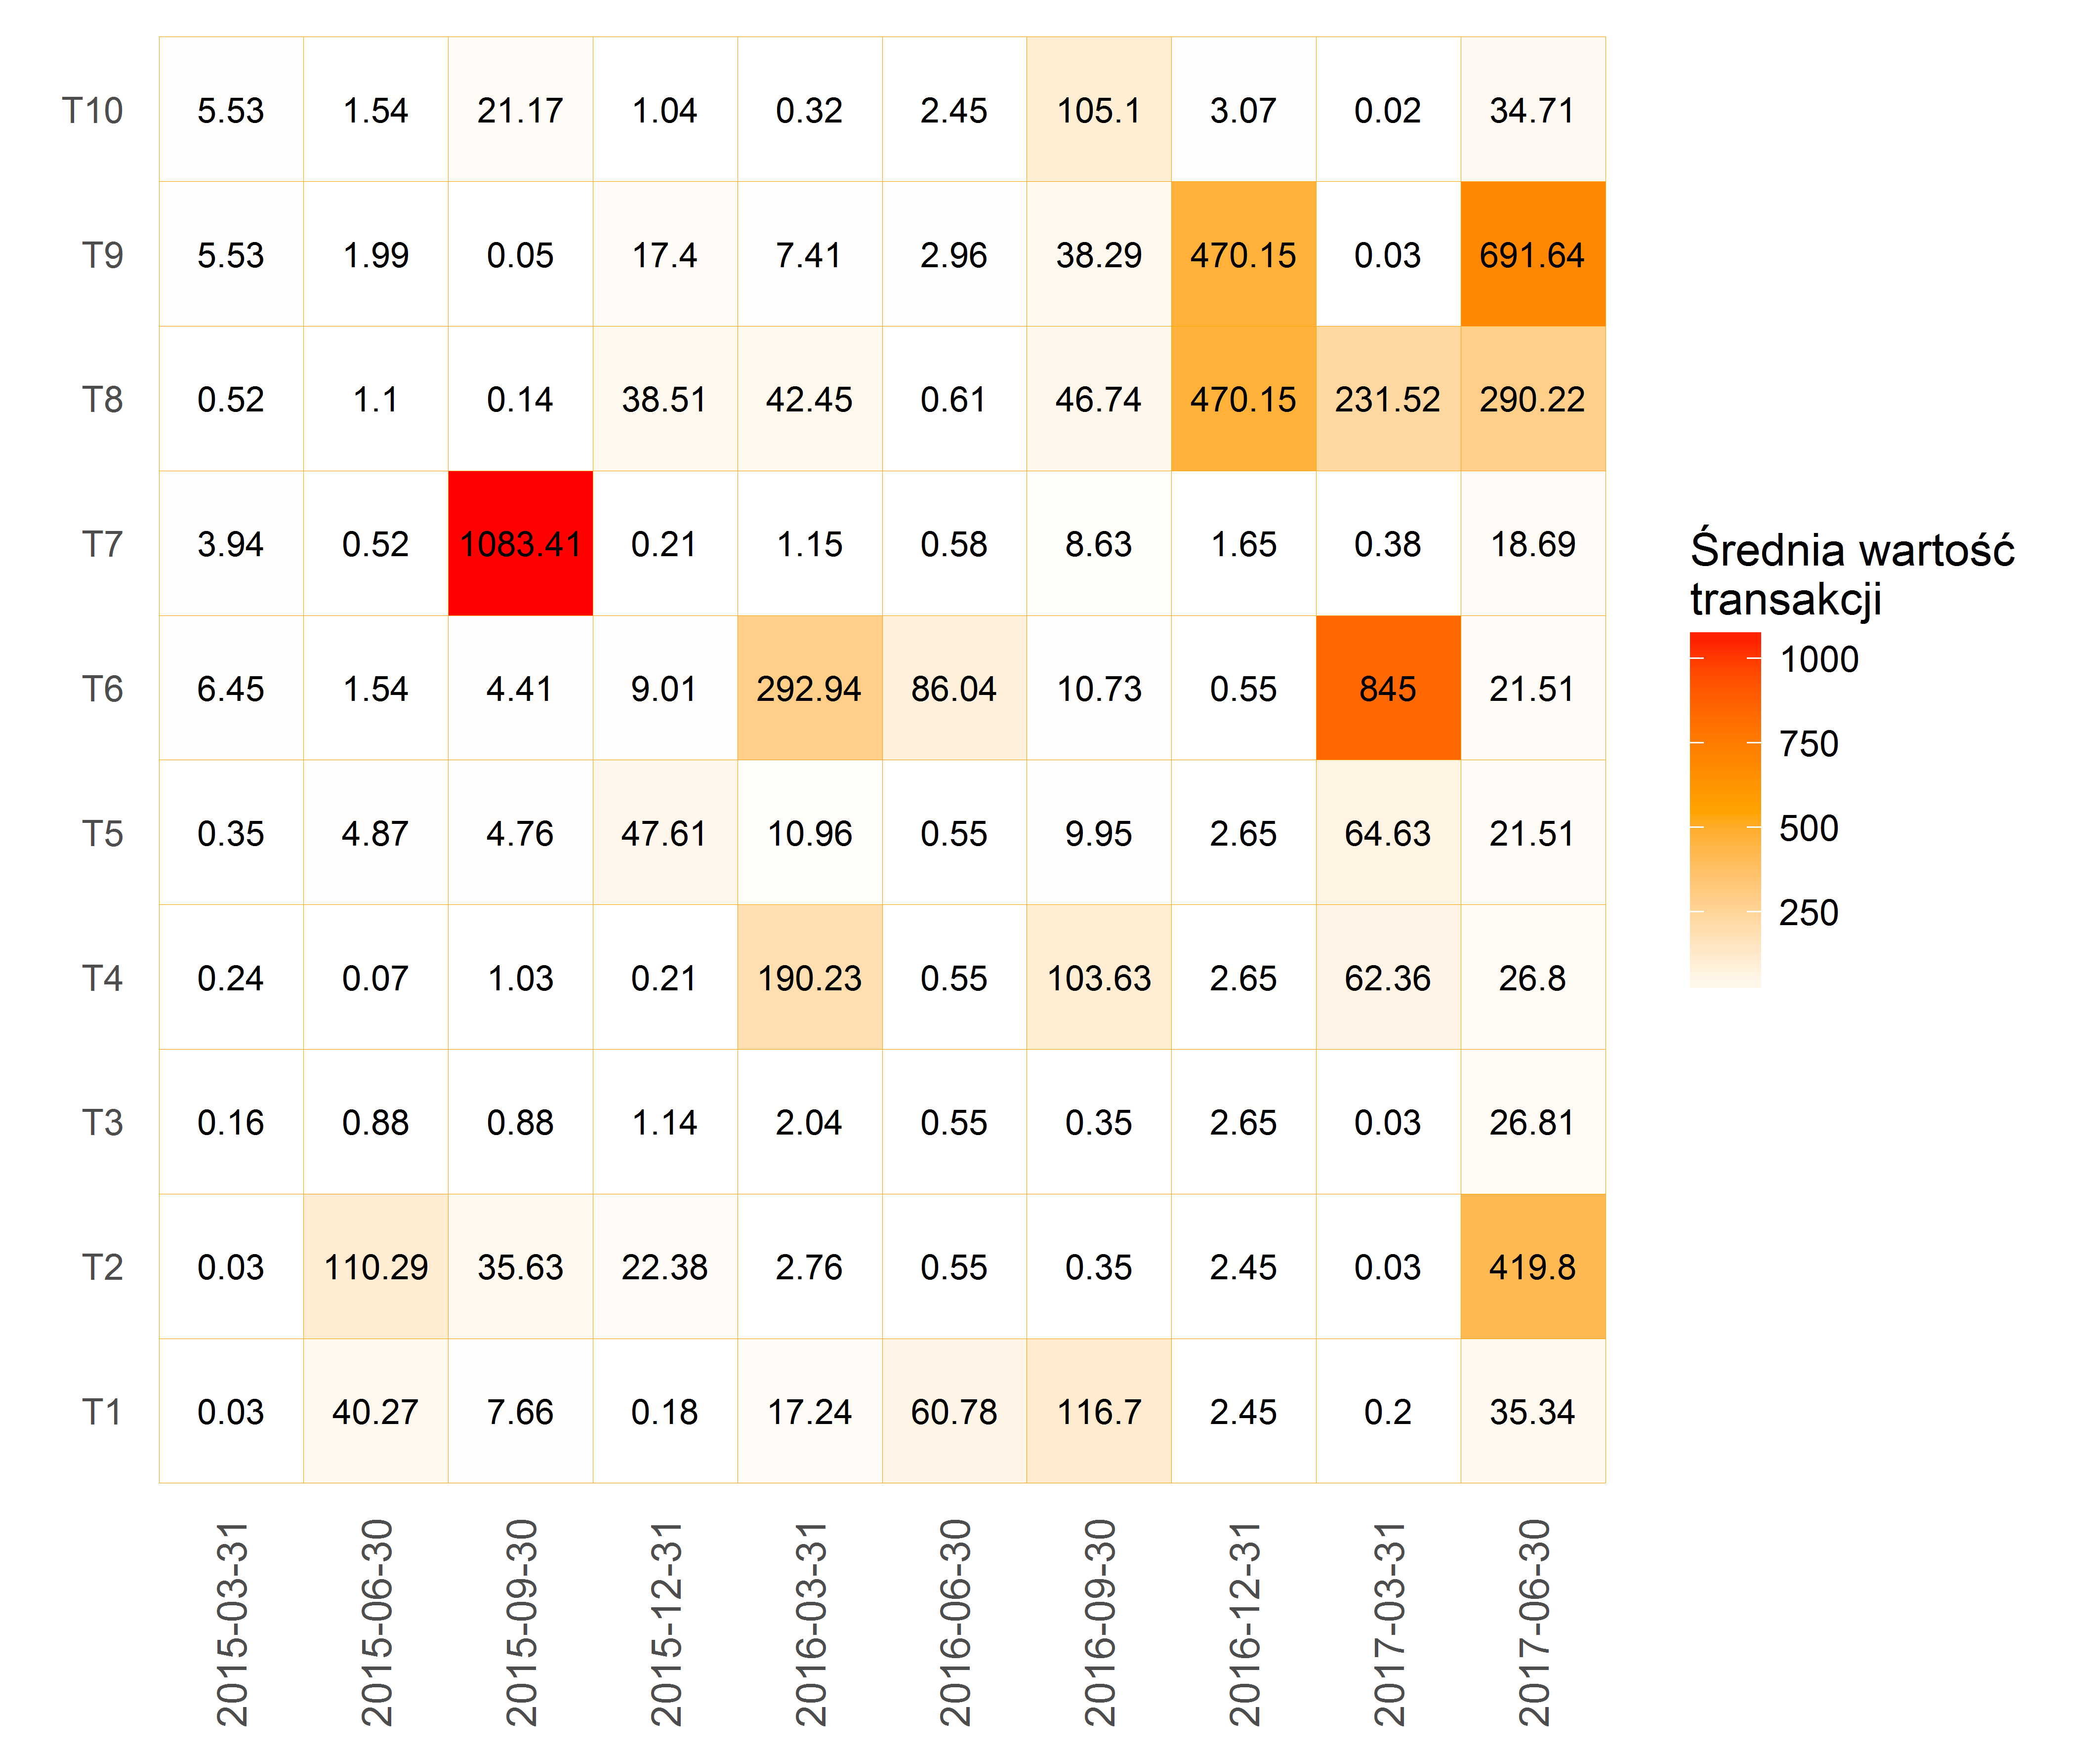
\includegraphics[width=\sizequad\textwidth]{pictures/wartosc_transakcji/wartosc_transakcji_hm.png}\quad  
  		 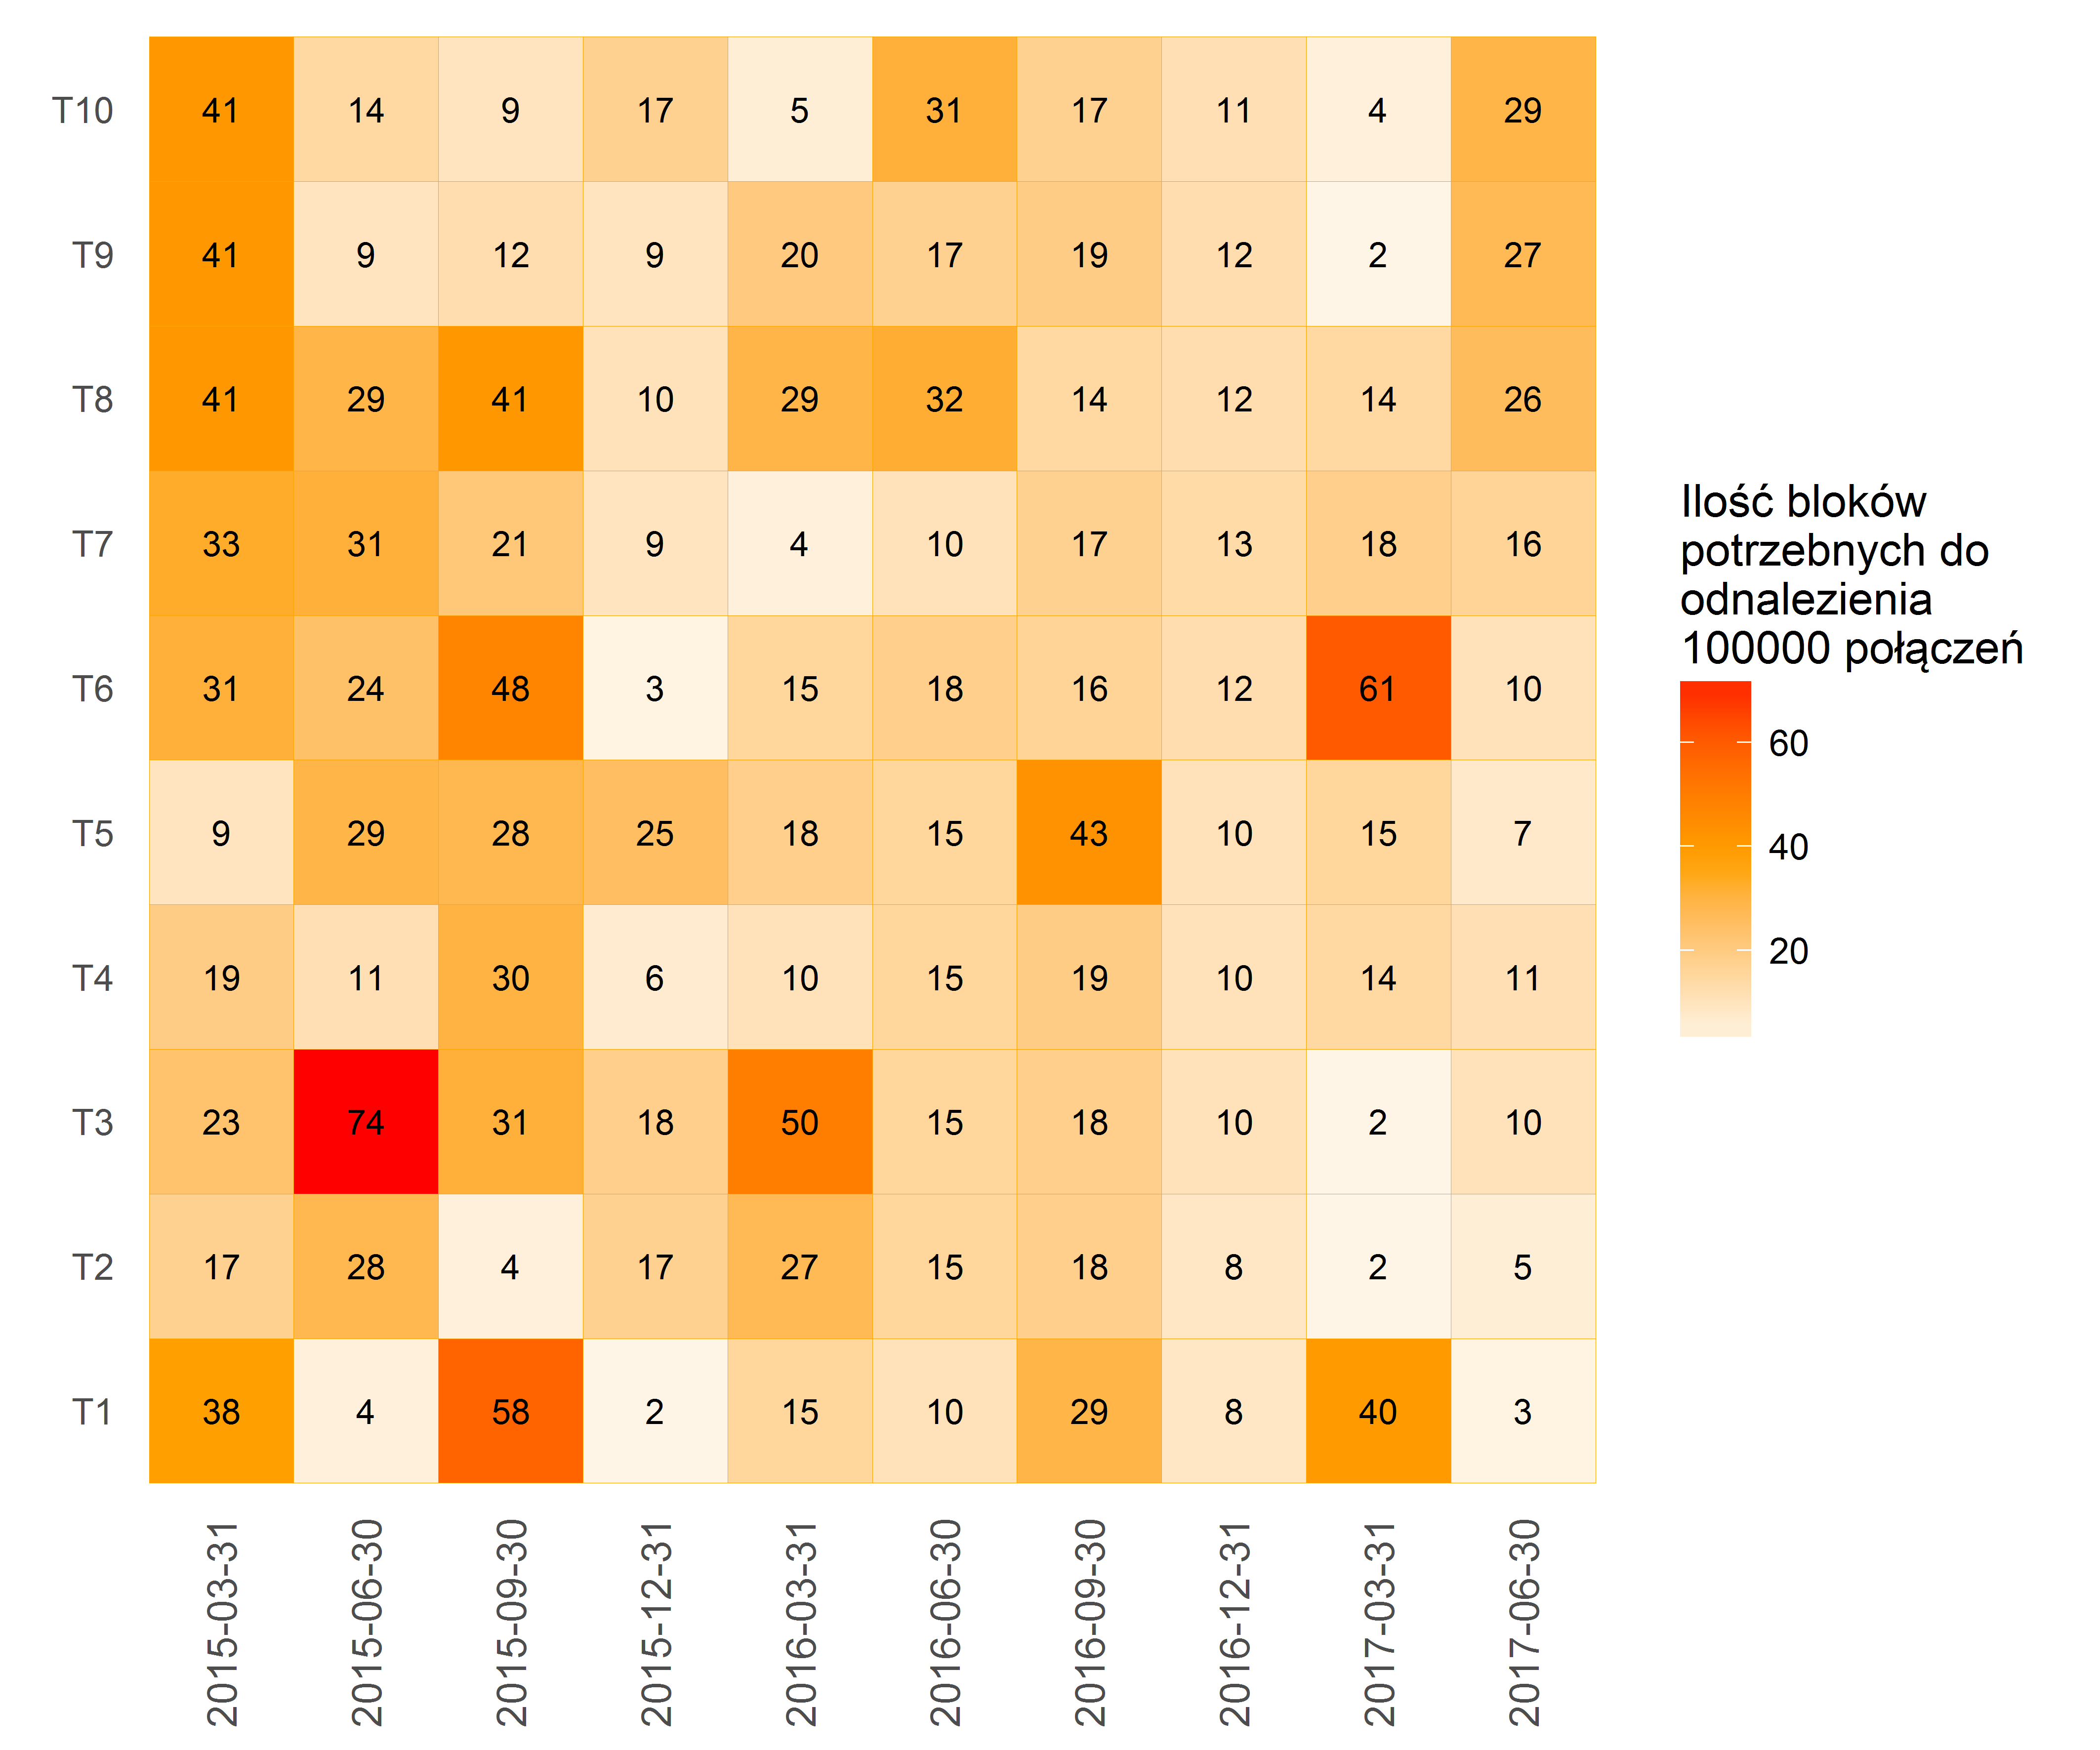
\includegraphics[width=\sizequad\textwidth]{pictures/ilosc_blokow/ilosc_blokow_hm.png}  \\
  		 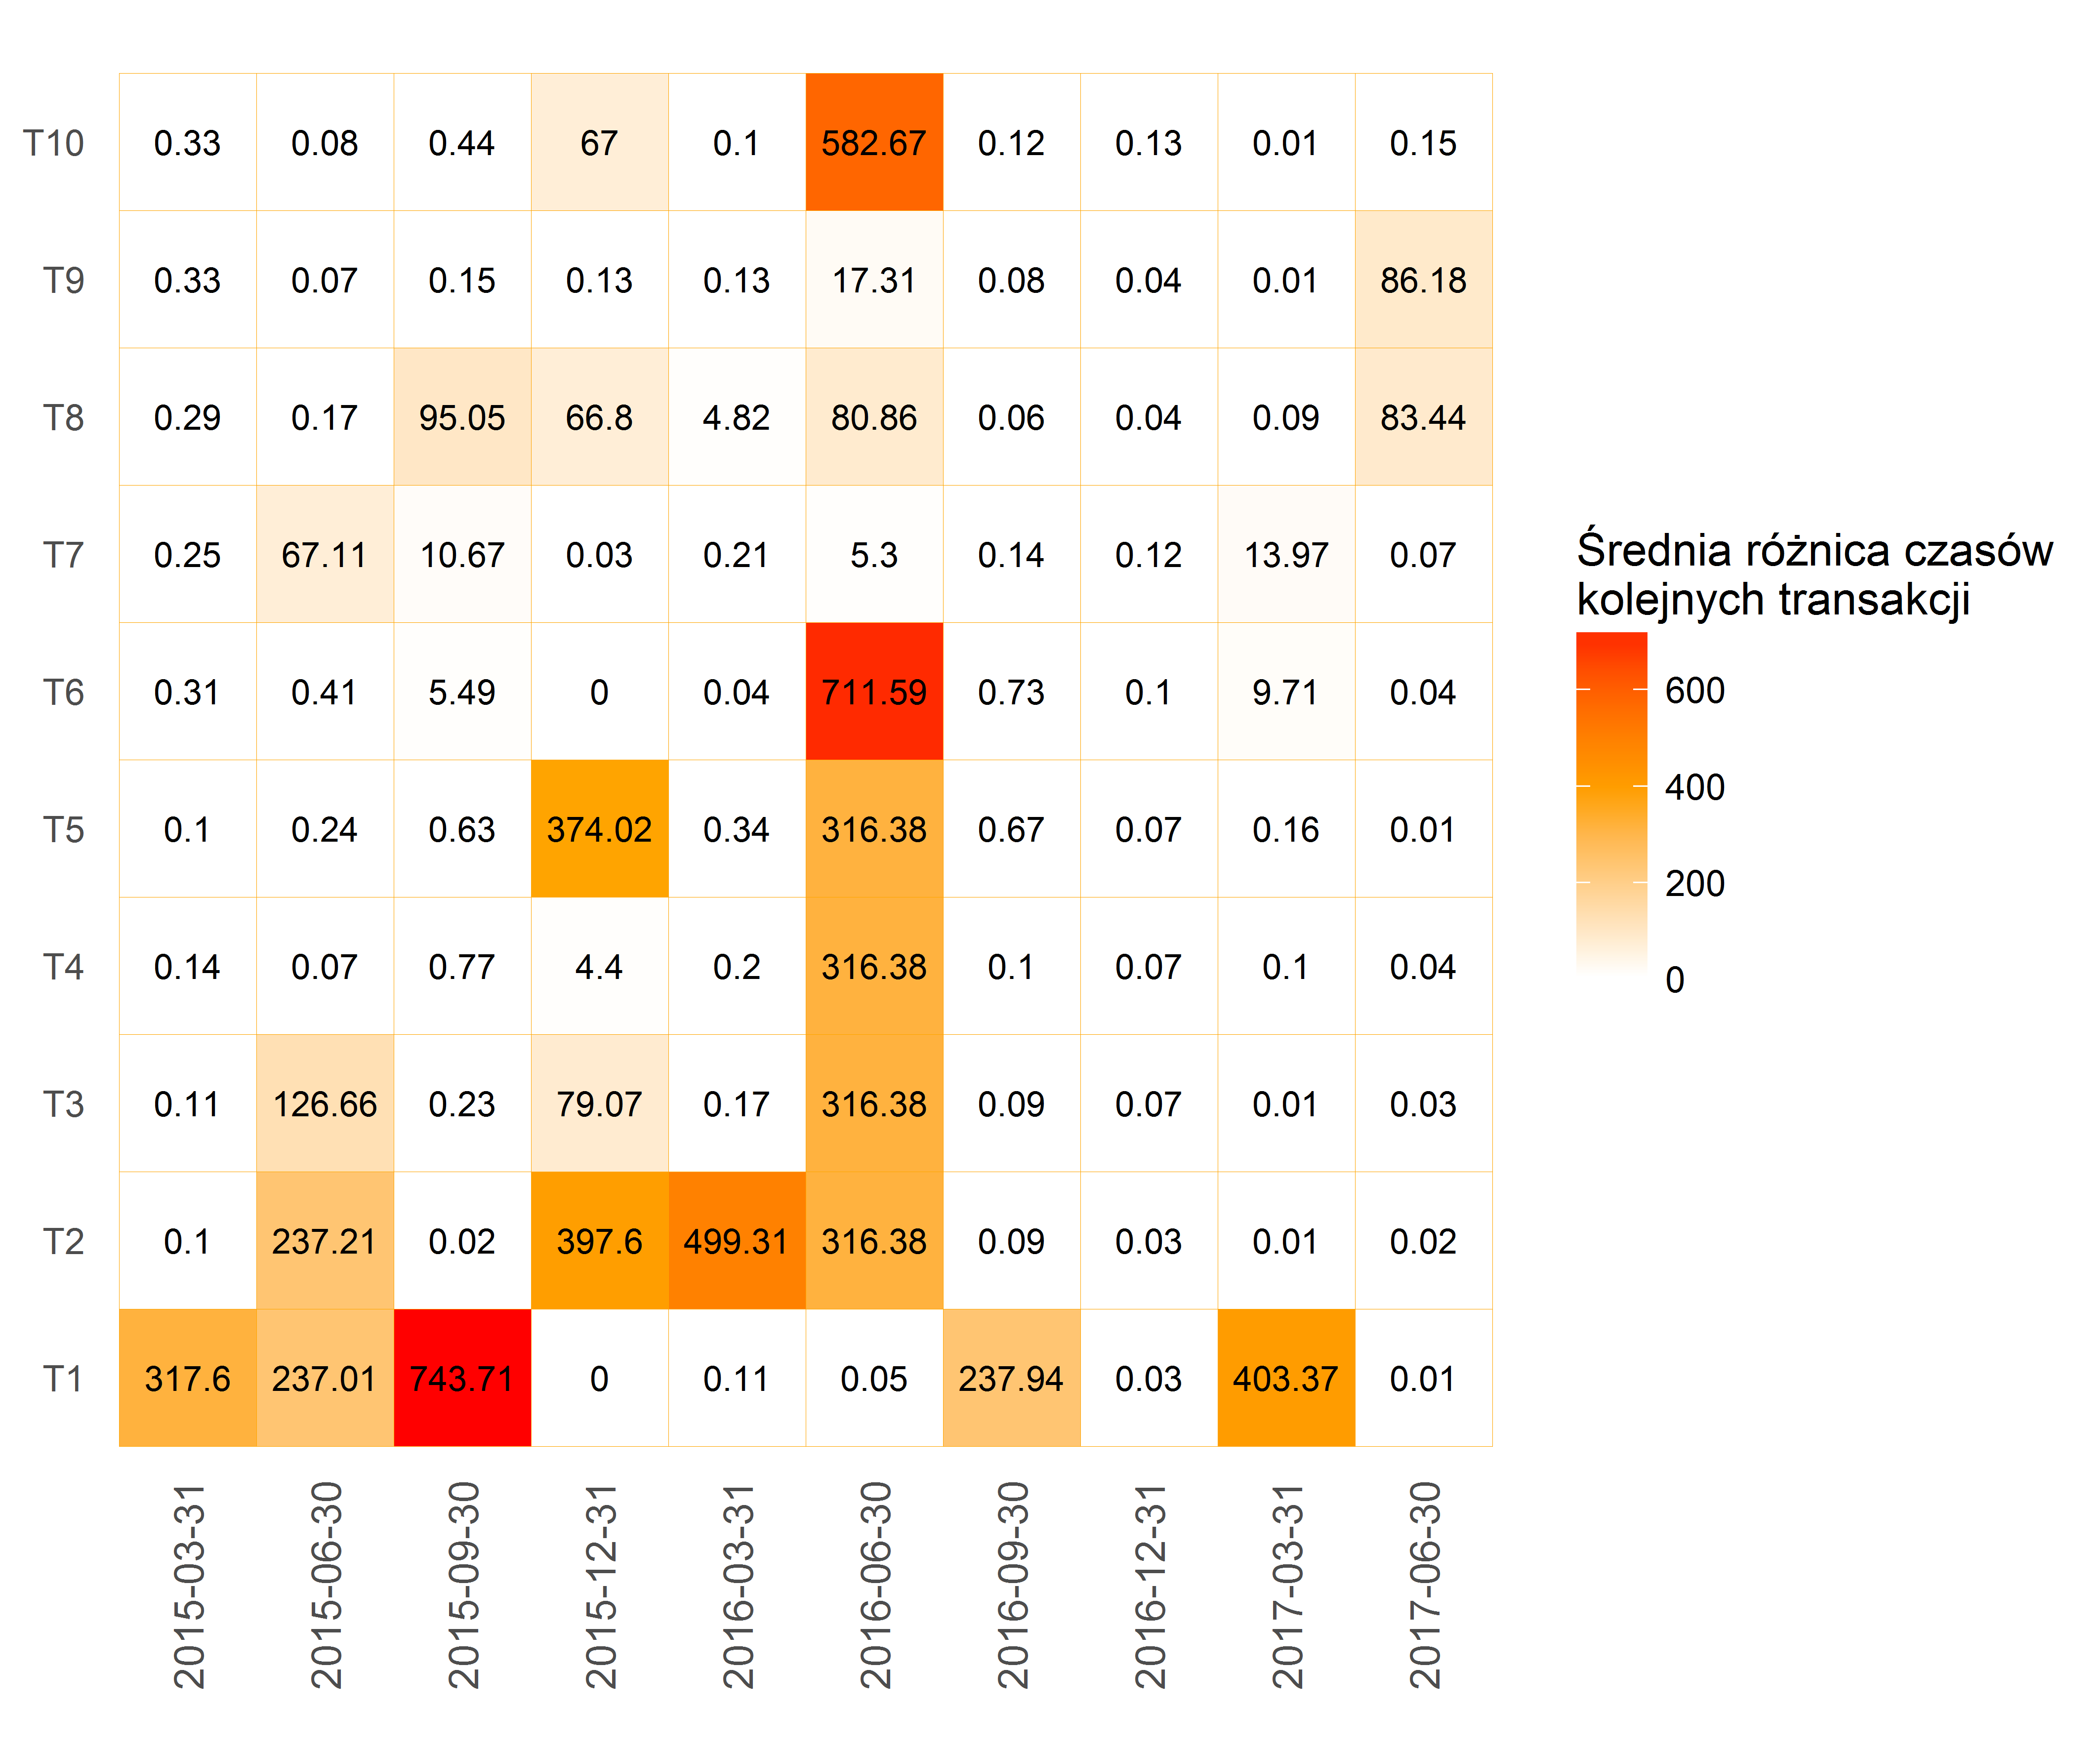
\includegraphics[width=\sizequad\textwidth]{pictures/roznica_czasow/roznica_czasow_hm.png}\quad
  		 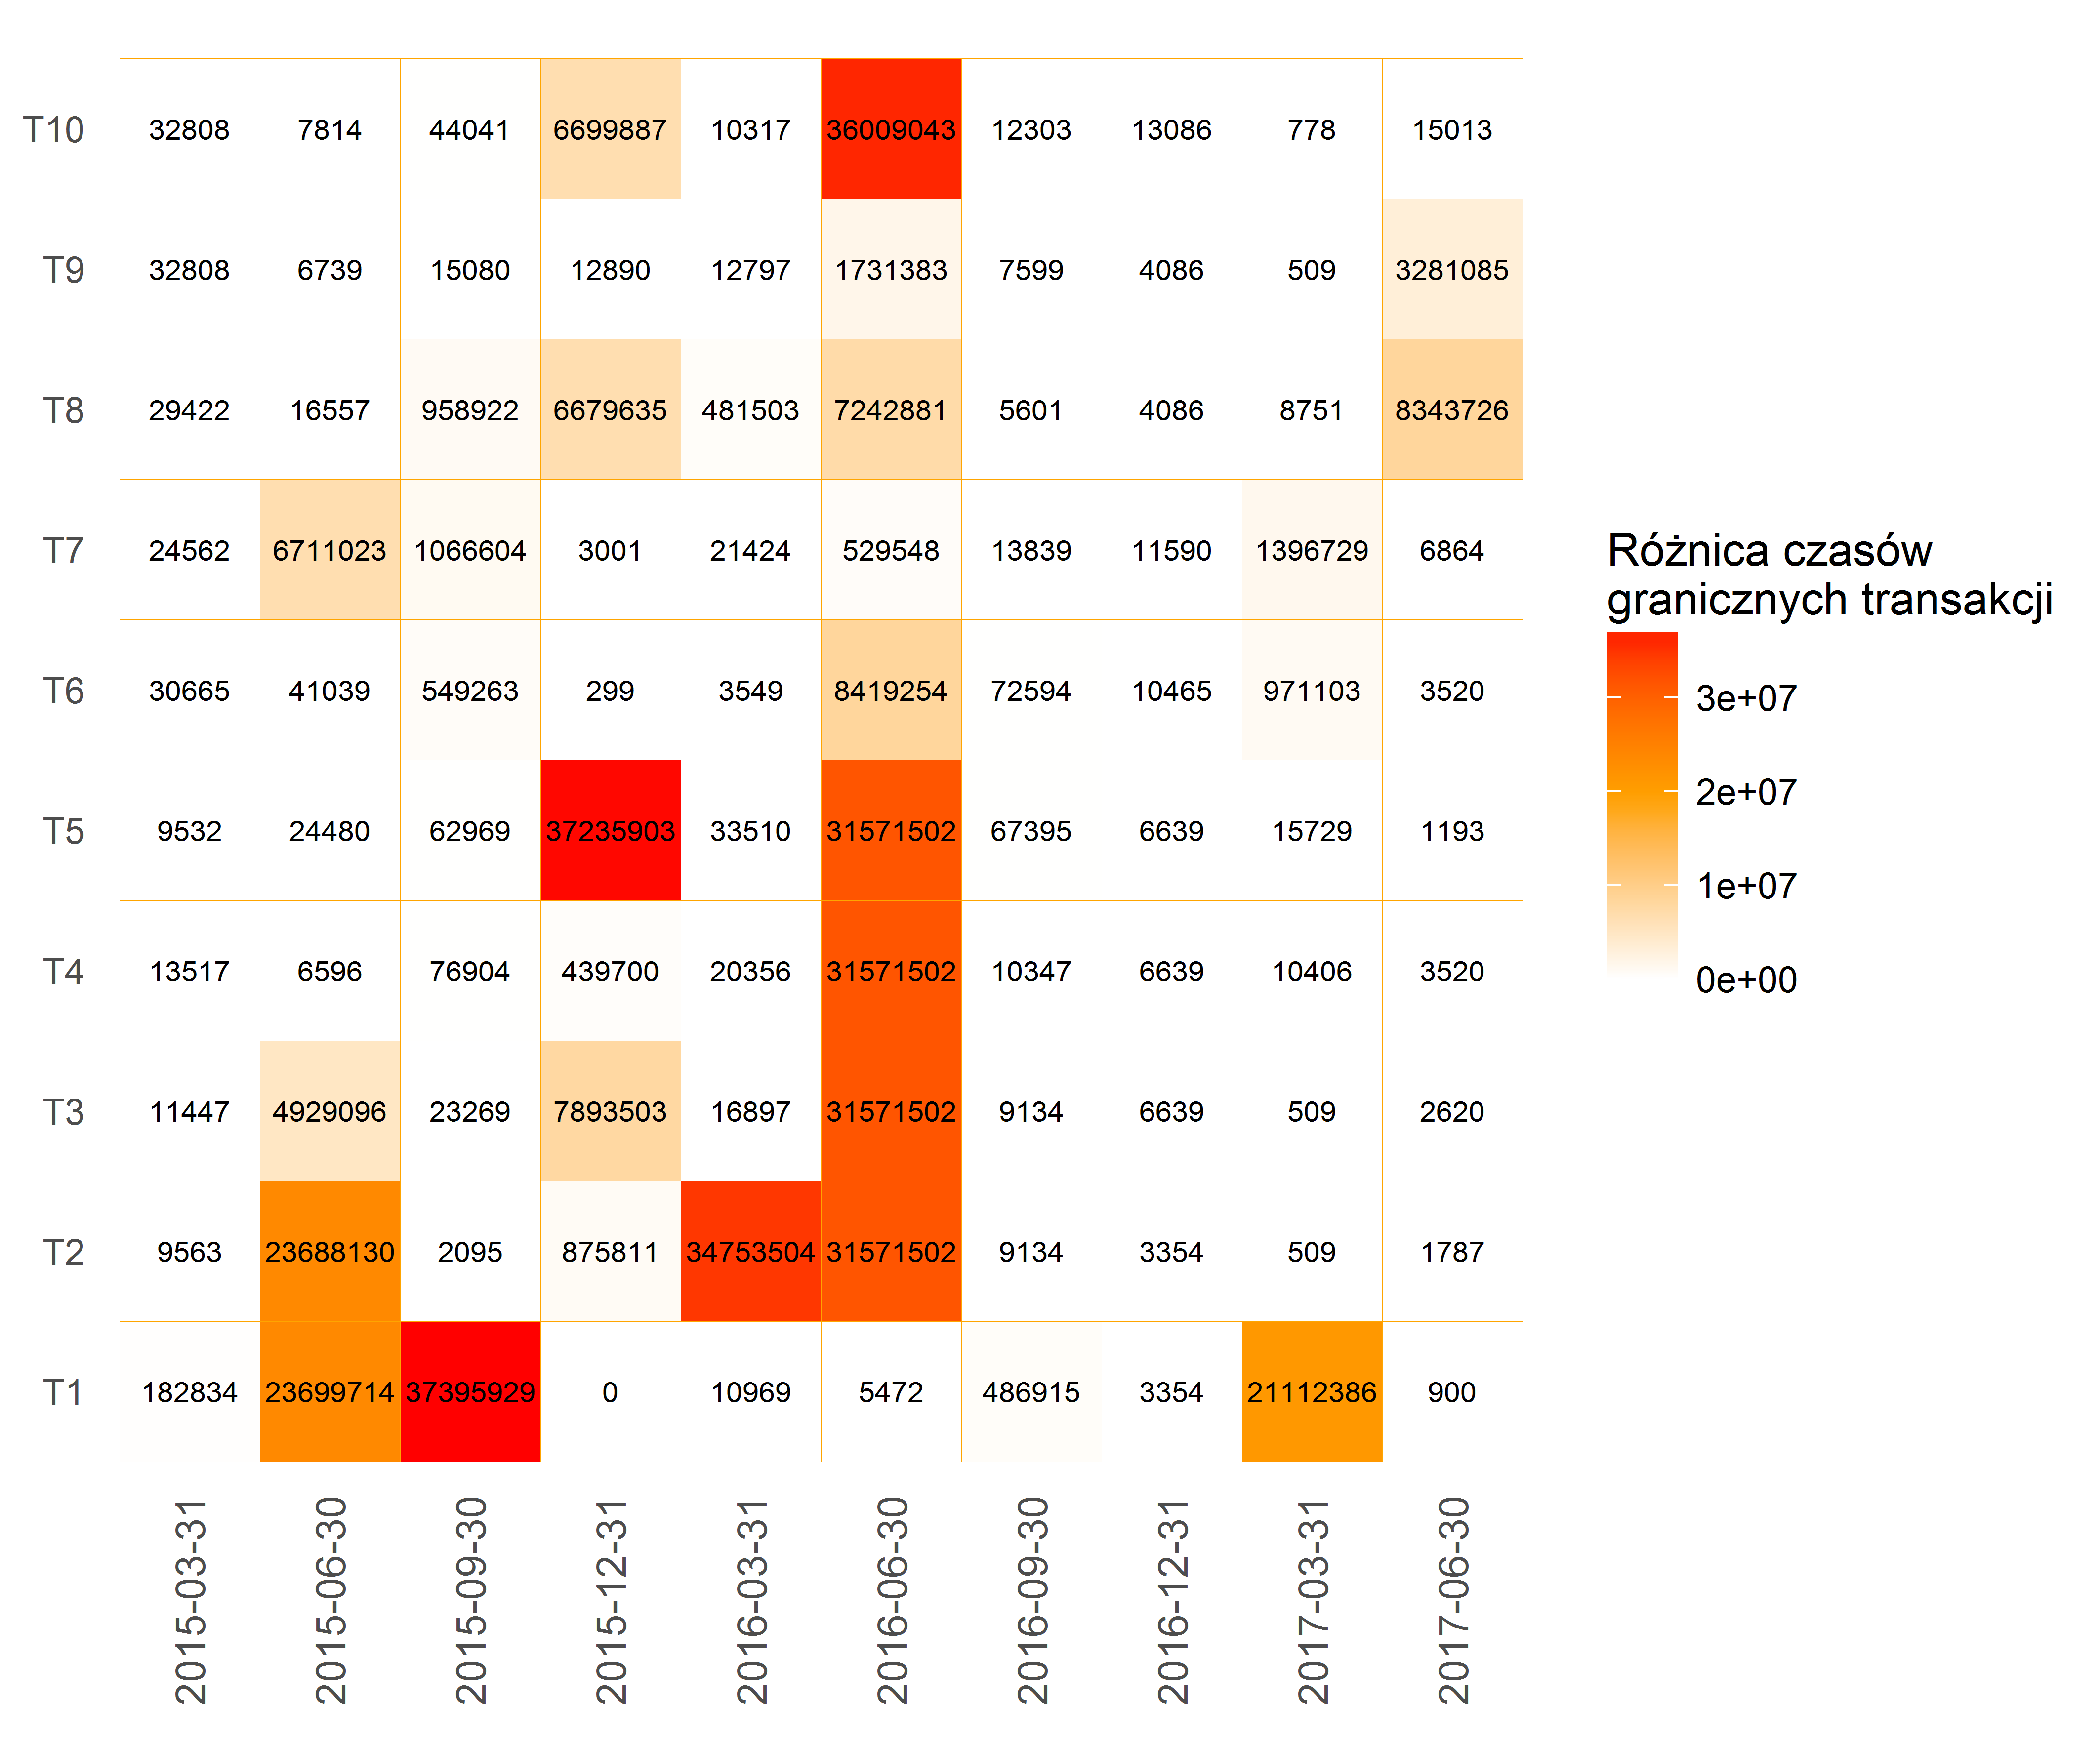
\includegraphics[width=\sizequad\textwidth]{pictures/czas_graniczny/czas_graniczny_hm.png}
 \end{minipage} 
\end{frame}

\begin{frame}
 \frametitle{Trend}
 \framesubtitle{Własności sieci wynikające z jej specyfiki}
    \begin{minipage}{\textwidth}
 		  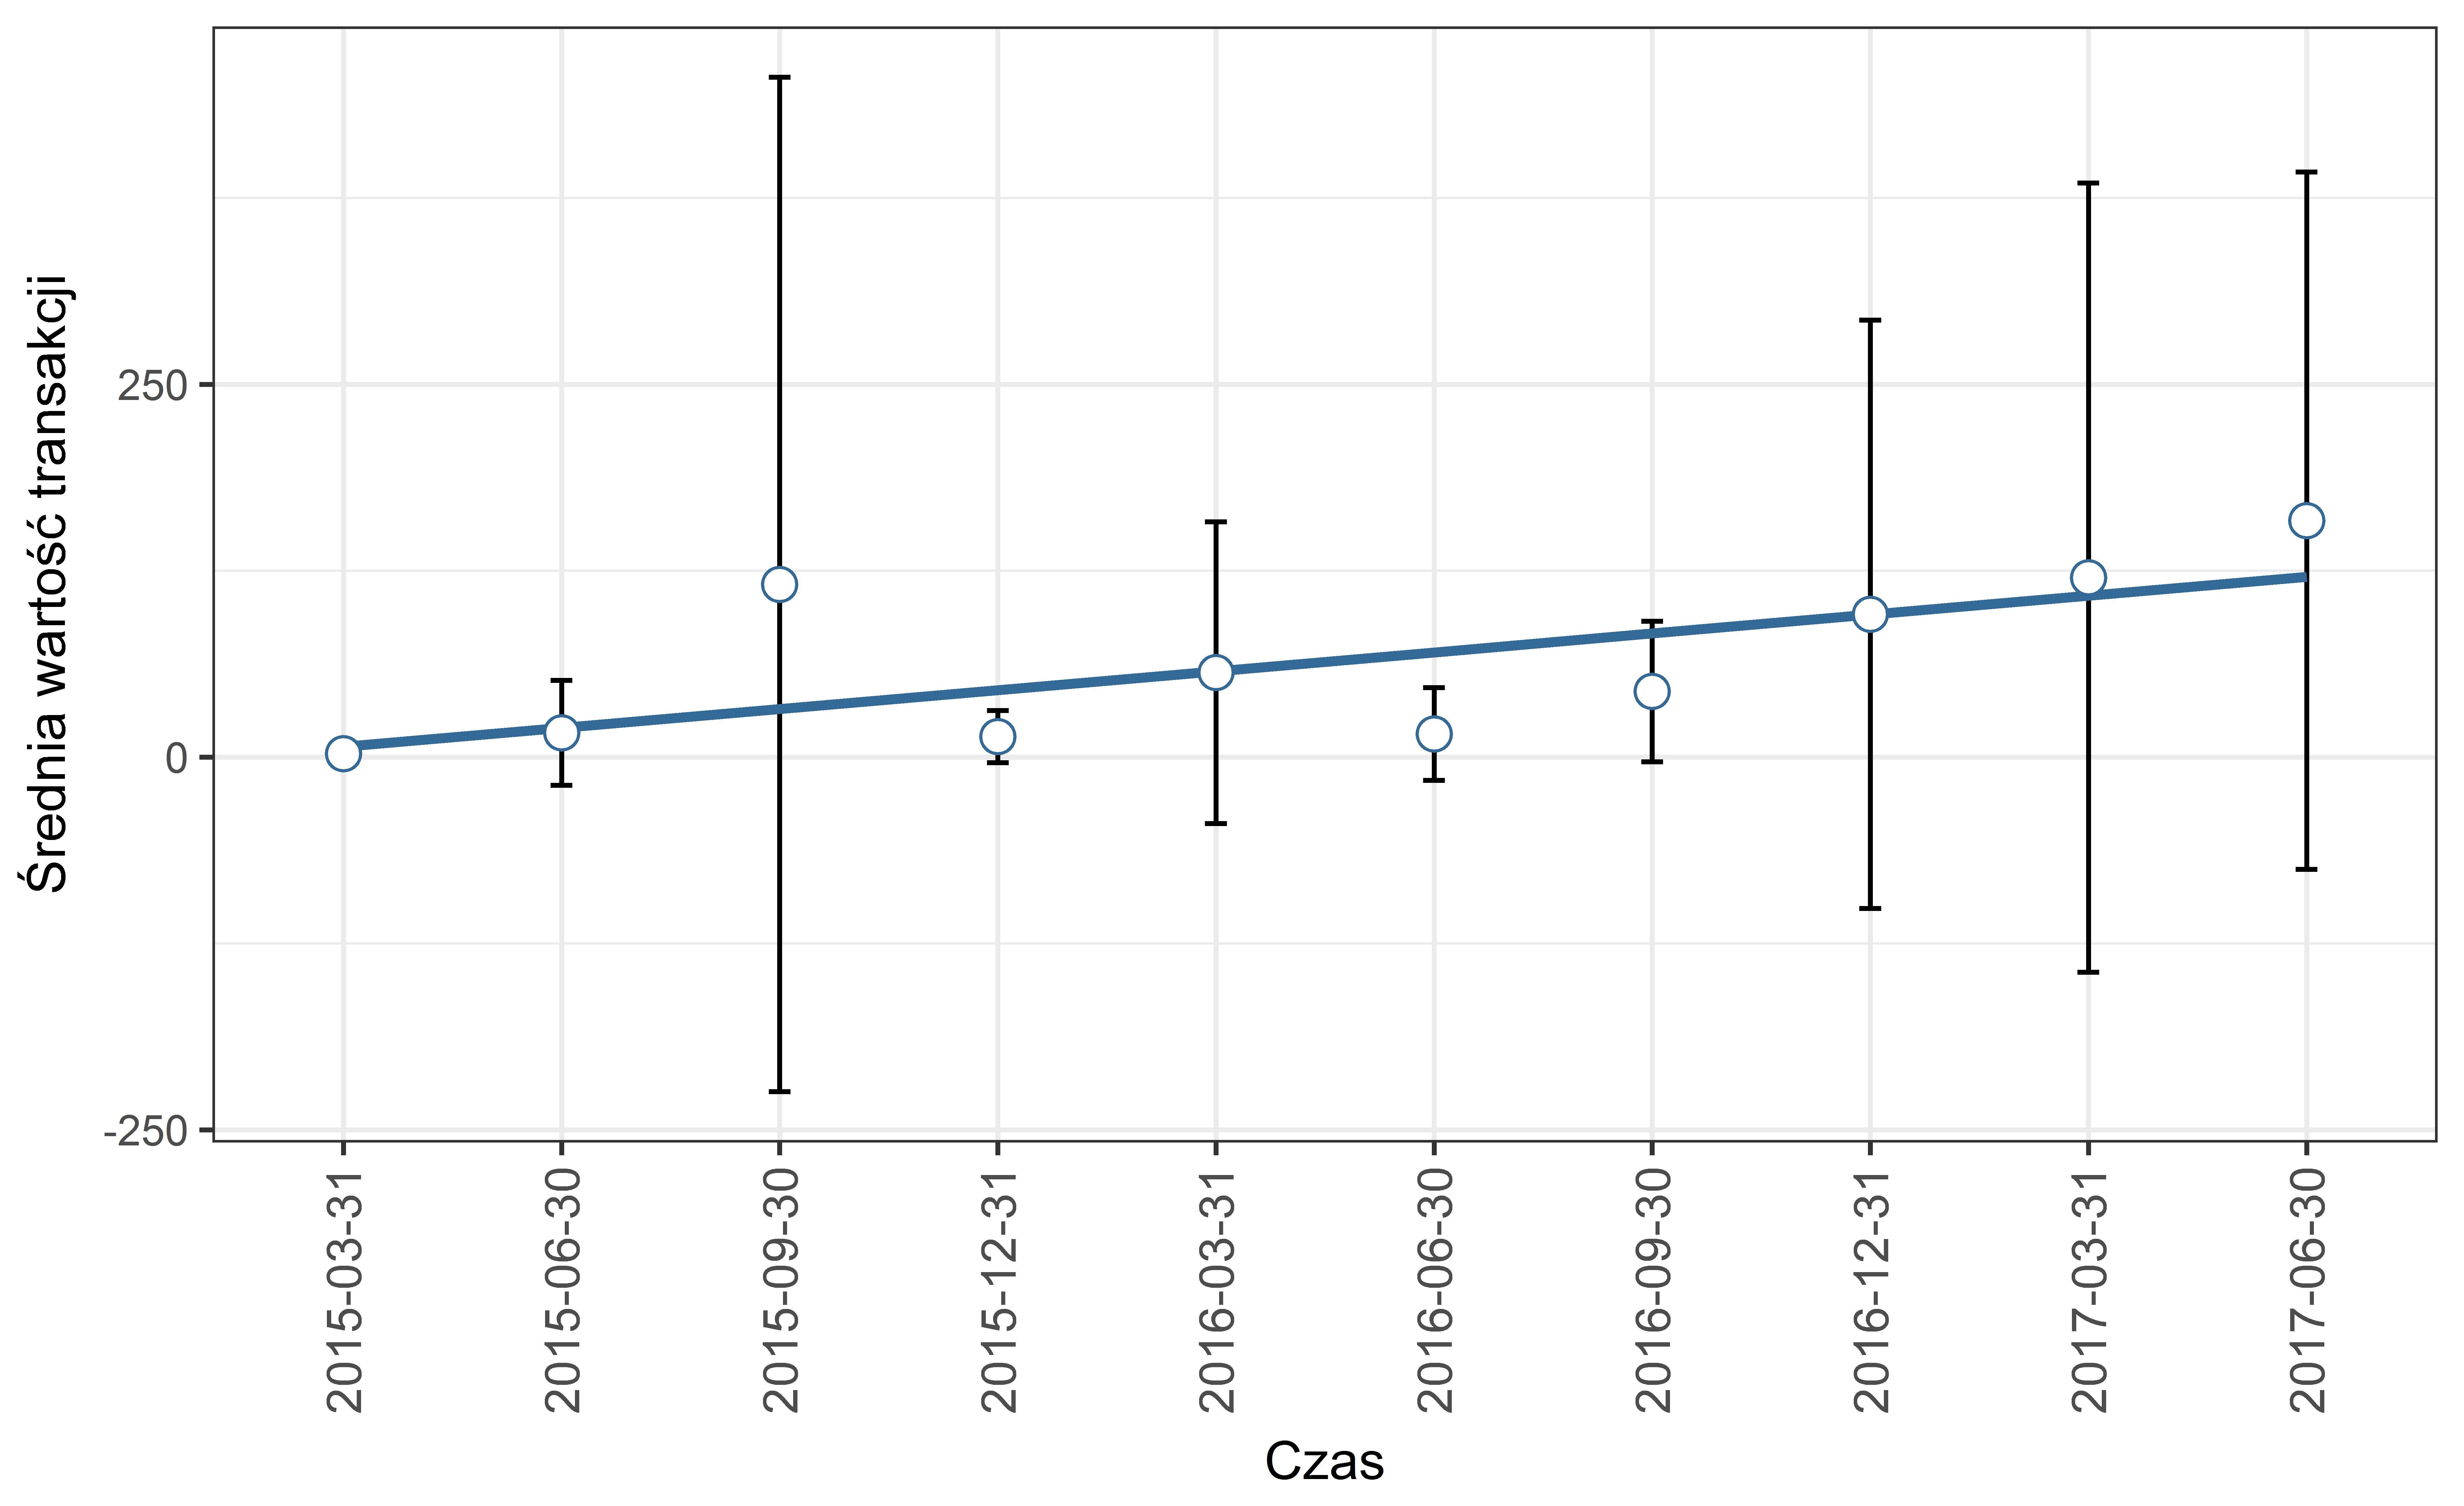
\includegraphics[width=\sizequadsda\textwidth]{pictures/wartosc_transakcji/wartosc_transakcji_sda.png}\quad  
  		 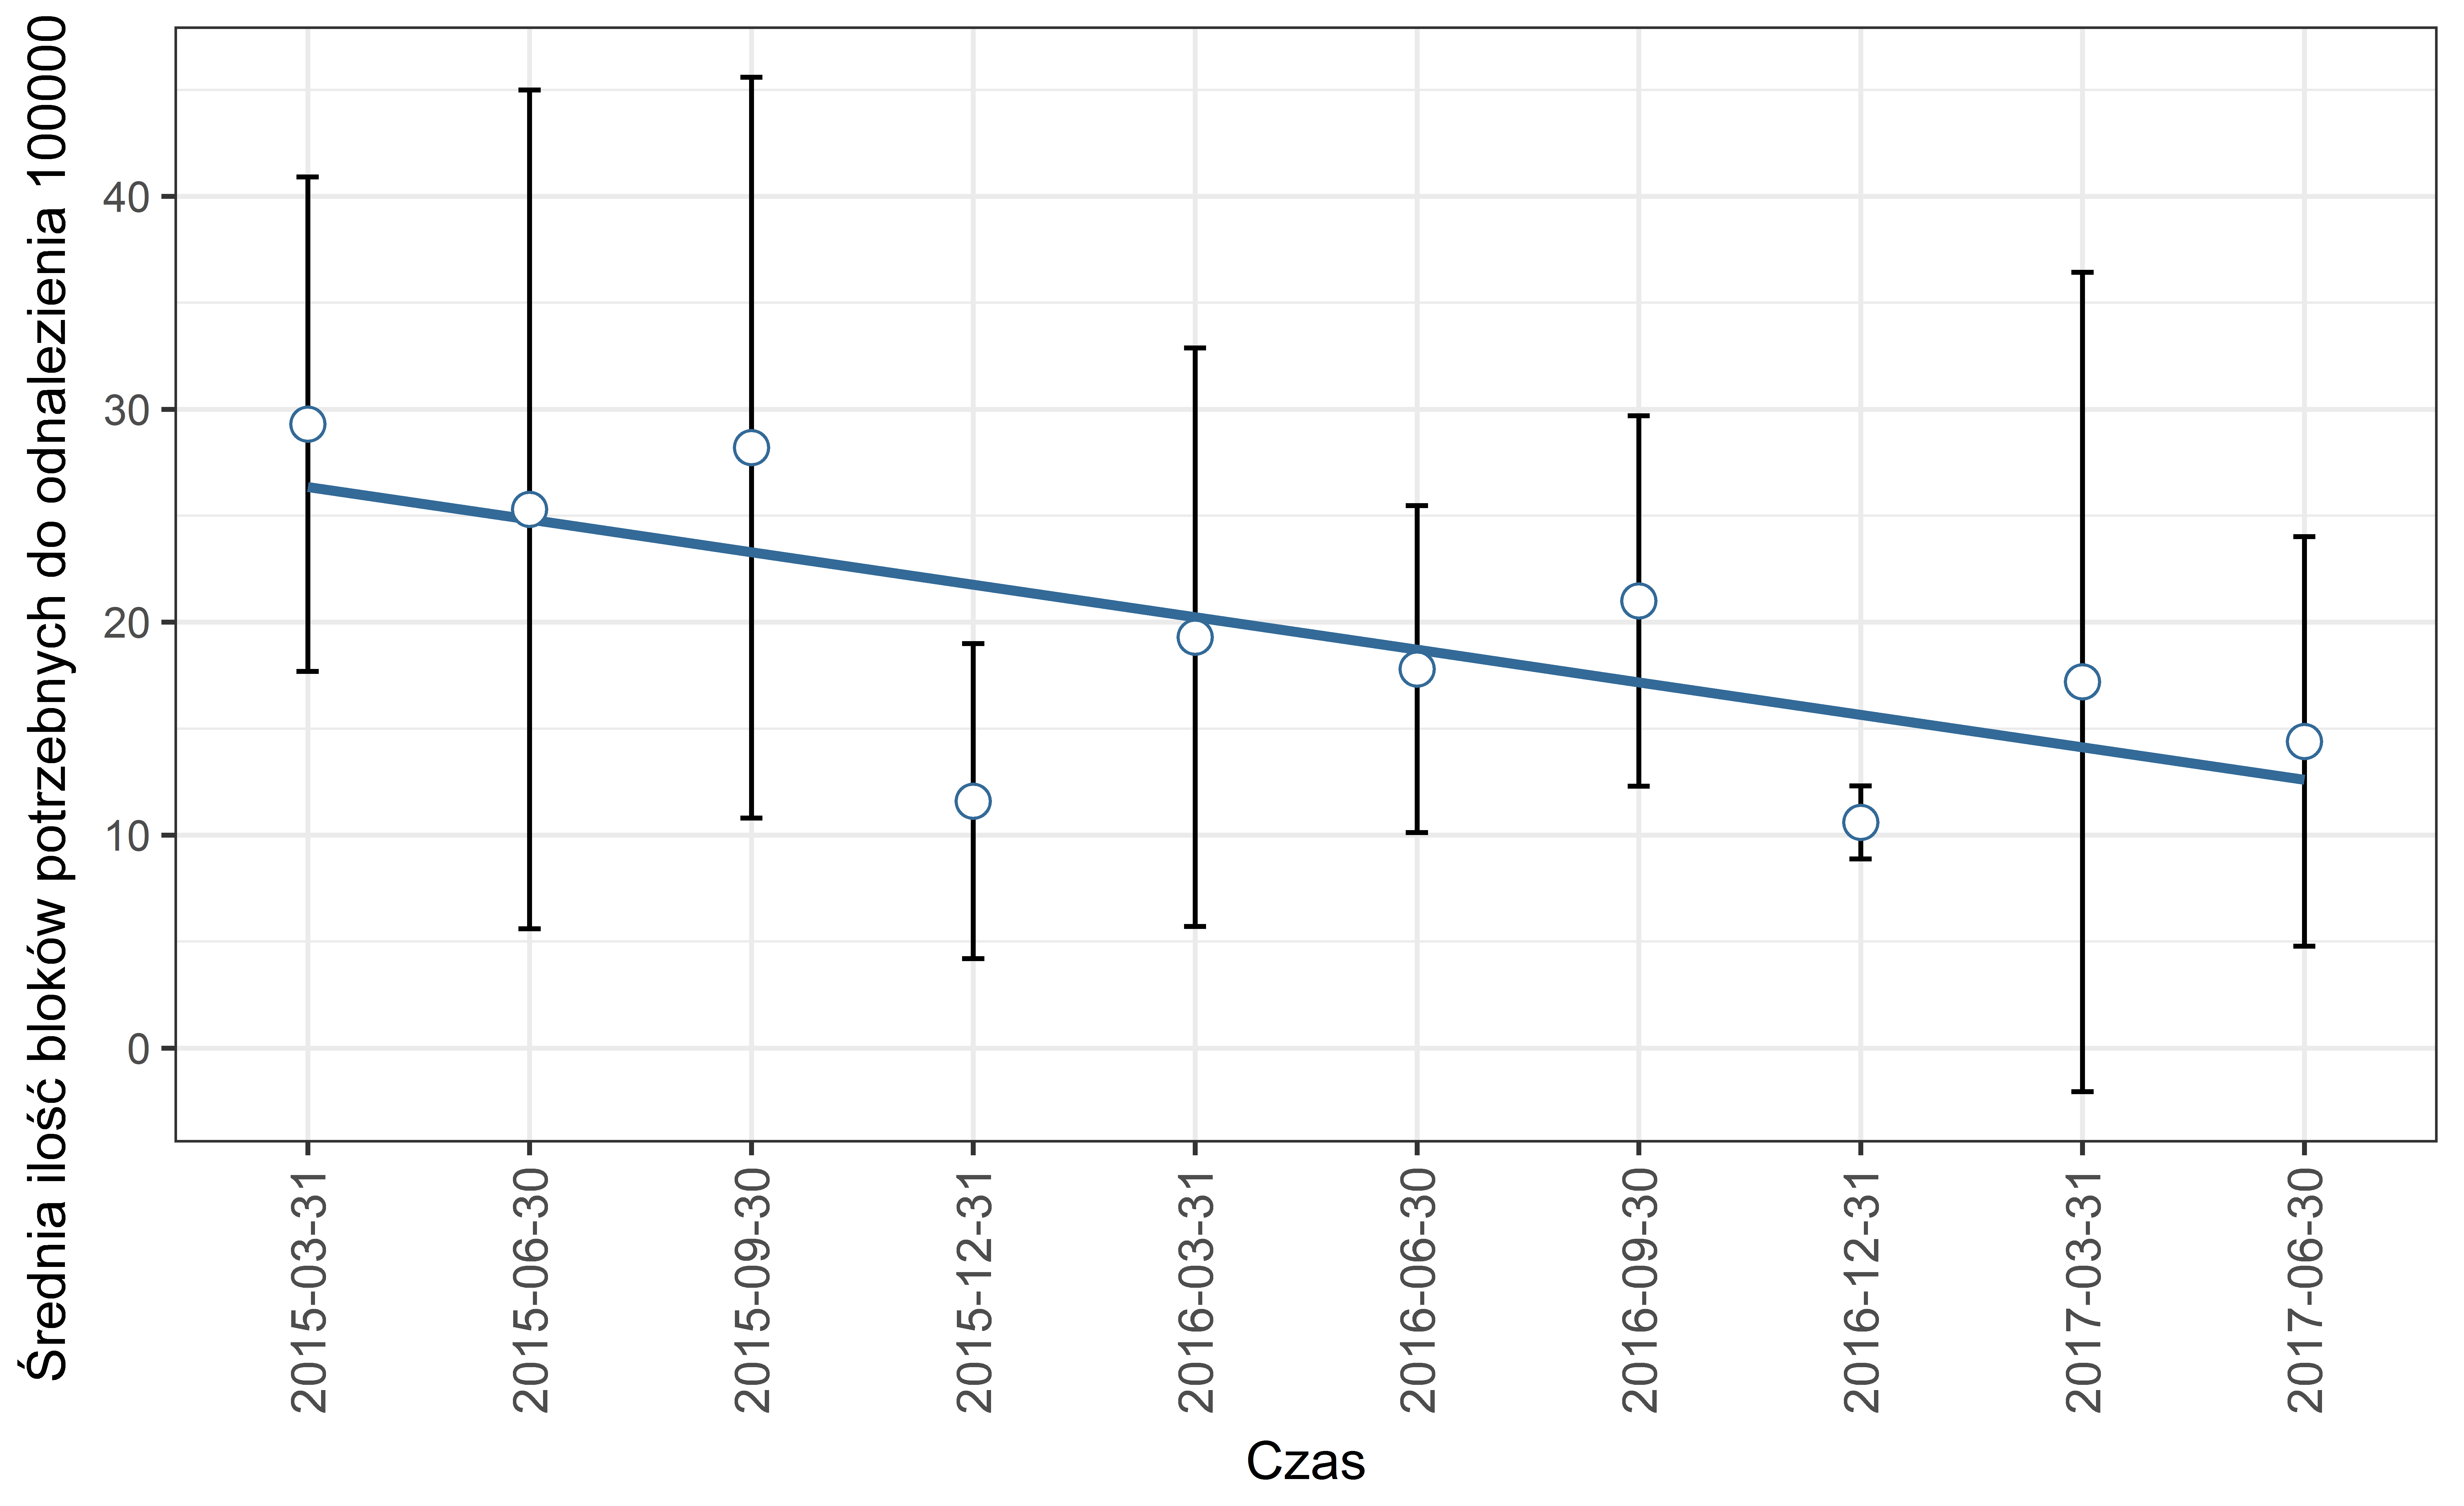
\includegraphics[width=\sizequadsda\textwidth]{pictures/ilosc_blokow/ilosc_blokow_sda.png}  \\
  		 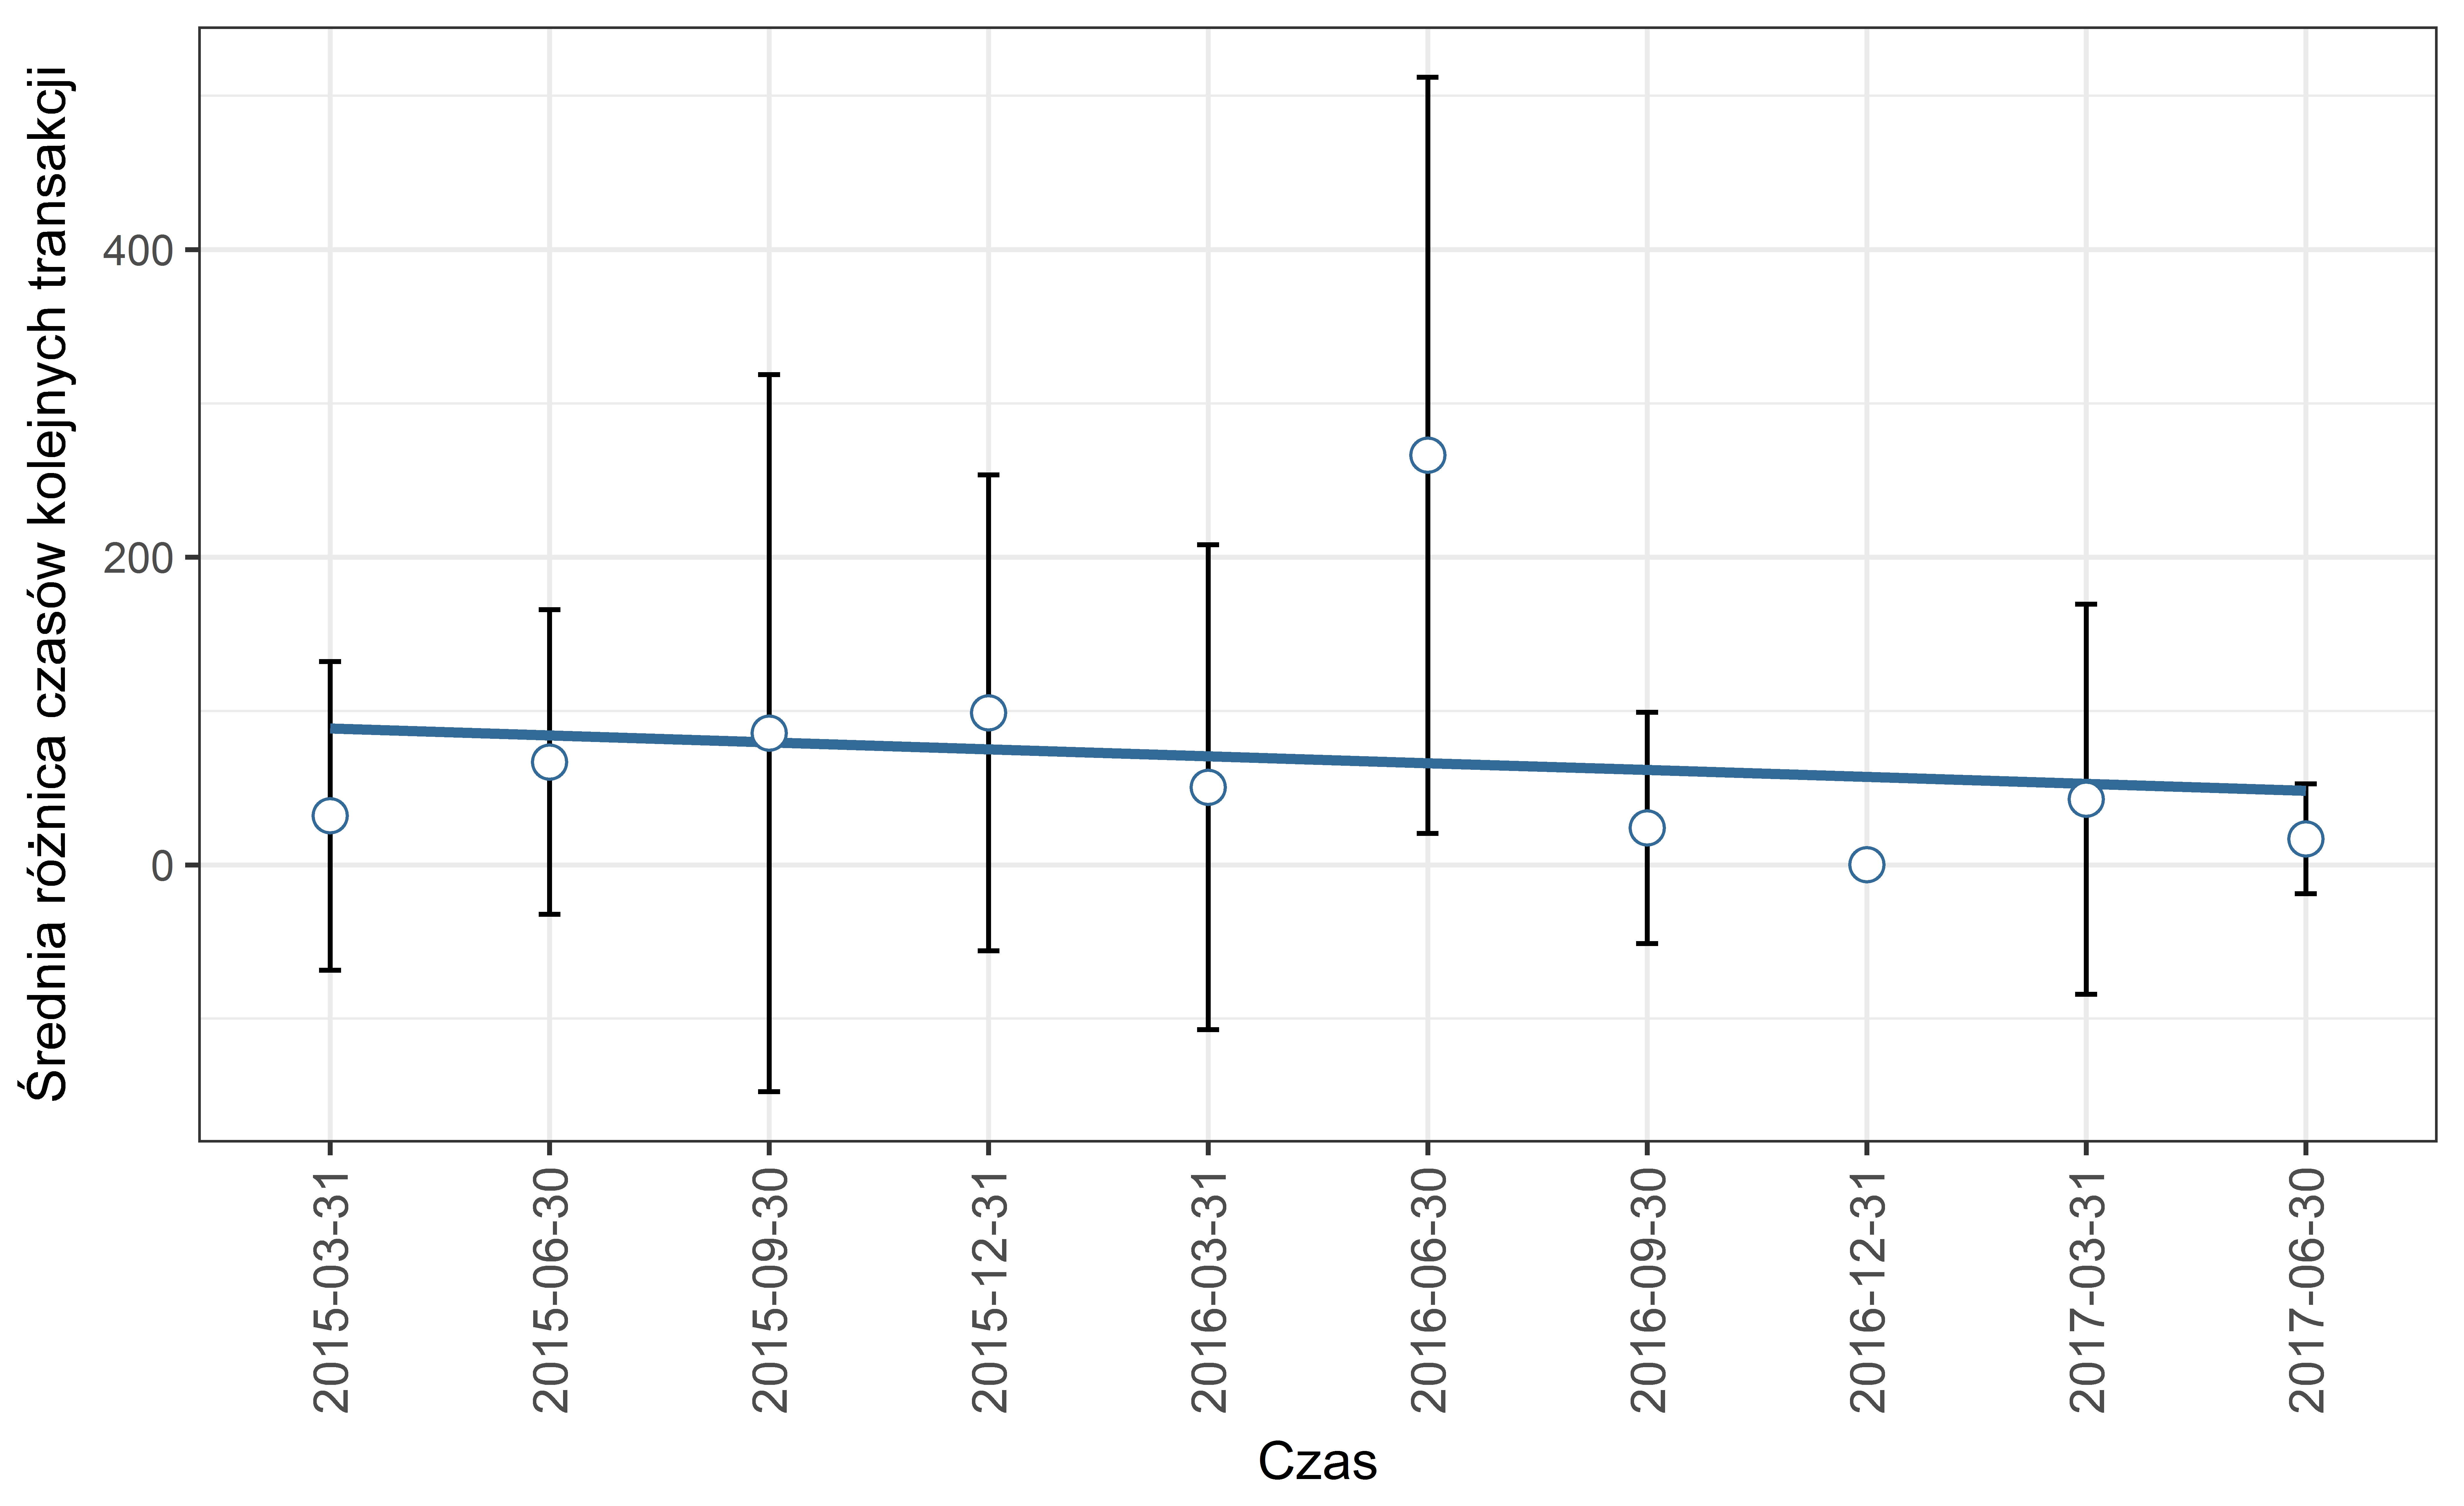
\includegraphics[width=\sizequadsda\textwidth]{pictures/roznica_czasow/roznica_czasow_sda.png}\quad
  		 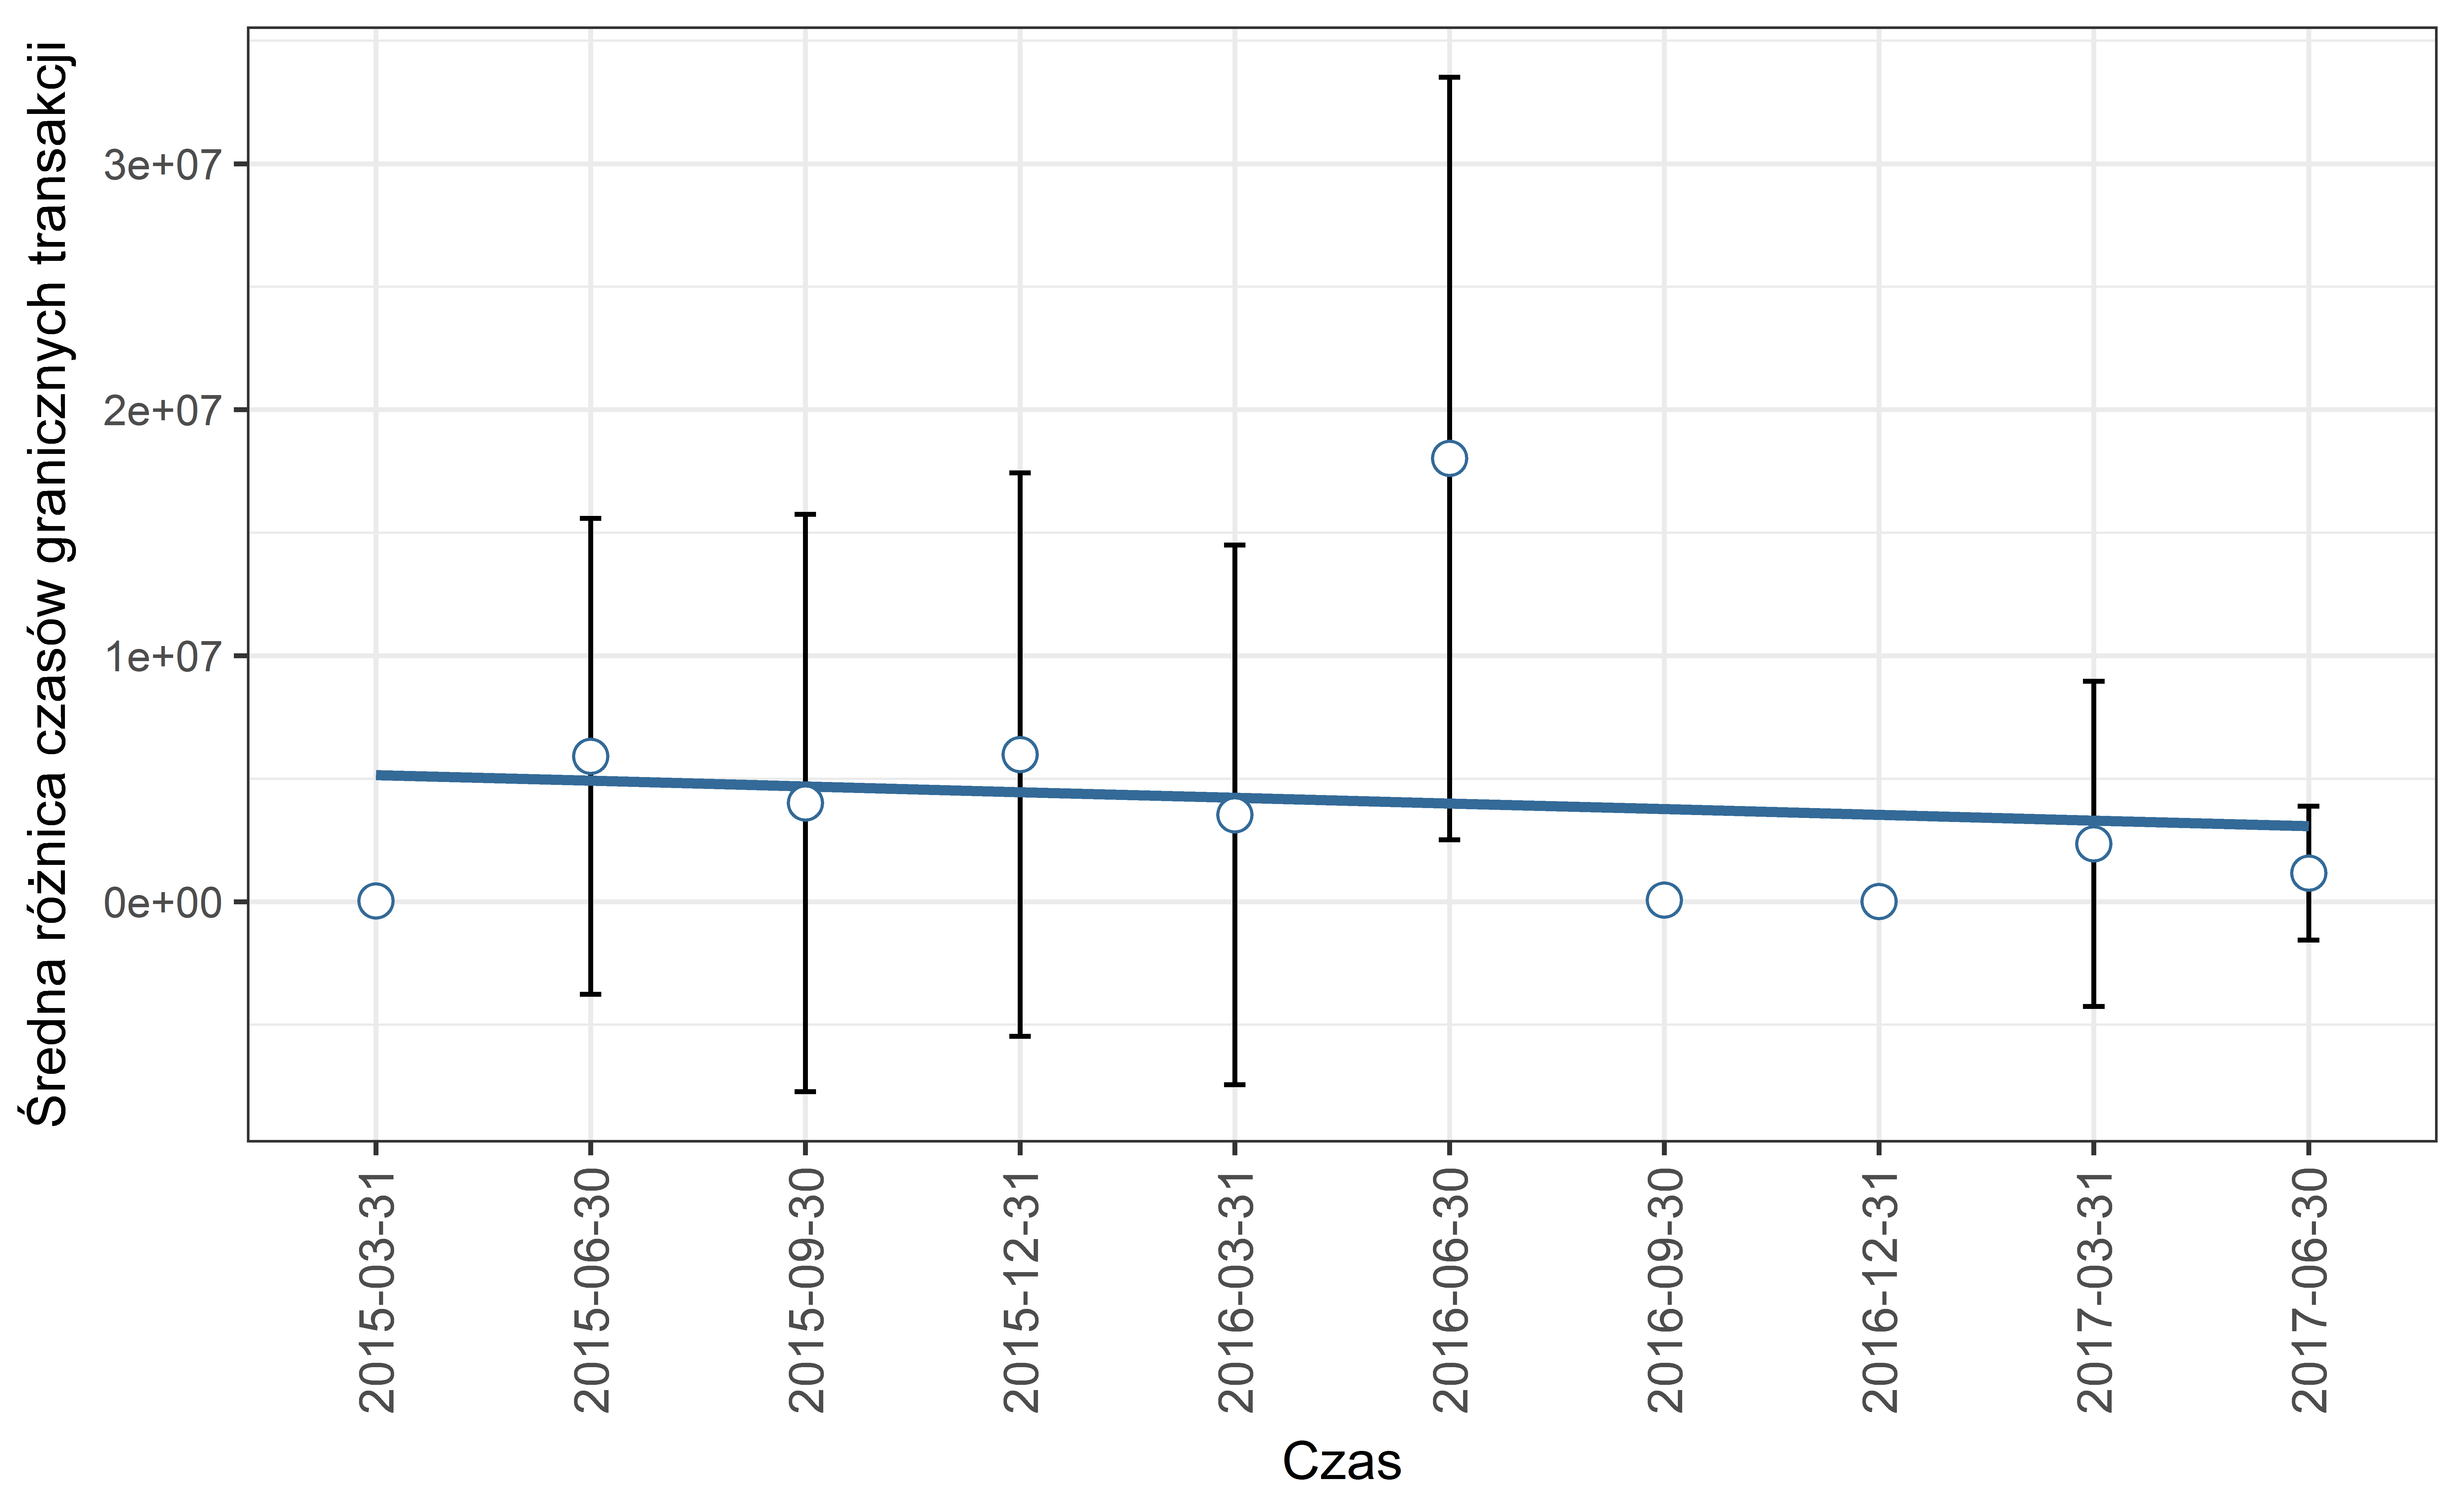
\includegraphics[width=\sizequadsda\textwidth]{pictures/czas_graniczny/czas_graniczny_sda.png}
  		  \end{minipage} 
\end{frame}


\begin{frame}
 \frametitle{Wnioski}
 \framesubtitle{}
 \begin{itemize}
 \item[A.] {\justifying{Sieć Bitcoin jest bardzo złożoną, dynamiczną i szybko rozwijającą się siecią.}\par} 
 \item[B.] {\justifying{Gęstość sieci rośnie, co w odniesieniu do jej specyfiki oznacza coraz większą ilość zlecanych transakcji, powstawanie dużej ilości nowych adresów oraz wzrost realizowanych transakcji pomiędzy różnymi uczestnikami sieci.}\par}
 \item[C.] {\justifying{Rosnąca ilość wykonywanych transakcji powoduje spadek istotności pojedynczej transakcji w całej sieci.}\par}
 \item[D.] {\justifying{Właściwości sieci nie są stałe w~jednym okresie, a~zależeć mogą od aktywności poszczególnych uczestników, dlatego też ilość połączeń pomiędzy transakcjami może być bardzo zróżnicowana.}\par}

  \end{itemize}
\end{frame}

\begin{frame}
 \frametitle{Wnioski}
 \framesubtitle{}
 \begin{itemize}
  \item[E.] {\justifying{Wartość większości transakcji nie przekracza 100 bitcoinów, a~zazwyczaj są to małe przekazy środków pomiędzy klientami sieci.}\par}
 \item[F.] {\justifying{Badanie ilości bloków potrzebnych do odnalezienia 100 tysięcy połączeń, w~powiązaniu z~analizą średniej różnicy czasów kolejnych transakcji oraz różnicy czasów transakcji granicznych jednoznacznie wskazuje na zwiększające się tempo rozwoju badanej sieci.}\par}
 \item[G.] {\justifying{Analiza znaczących wartości transakcji pozwoliła na powiązanie okresów z wzmożoną aktywnością giełd.}\par}
  \end{itemize}
\end{frame}

\end{document}